% \iffalse meta-comment
%
% Copyright (C) 2022 by Skippi \url{https://github.com/Skipp1/fortex}
% ---------------------------------------------------------------------------
% This work may be distributed and/or modified under the
% conditions of the LaTeX Project Public License, either version 1.3
% of this license or (at your option) any later version.
% The latest version of this license is in
%   http://www.latex-project.org/lppl.txt
% and version 1.3 or later is part of all distributions of LaTeX
% version 2005/12/01 or later.
%
% This work has the LPPL maintenance status `maintained'.
%
% The Current Maintainer of this work is Skippi.
%
% This work consists of the files fortex.dtx and fortex.ins
% and the derived filebase fortex.sty.
%
%
%<*driver>
\documentclass[cm-default, a4paper]{l3doc}
\usepackage[verbose, tmpdir=.]{fortex}
\usepackage{expl3}
\usepackage[UKenglish]{babel}
\usepackage[dvipsnames]{xcolor}
\usepackage{microtype}
\usepackage{tikz}
\usepackage{listings}
\usepackage{bookmark}
\usepackage[pass]{geometry}
\EnableCrossrefs
\lstset {
  gobble=3,
  language=[LaTeX]TeX,
  basicstyle=\small\ttfamily,
  numbers=left,
  firstnumber=1,
  numberfirstline=true, 
  tabsize=2,
  showstringspaces=false,
}
\NewDocumentEnvironment{examplefile}{v}{
  \noindent
  \begin{tikzpicture}[overlay]
    \draw[rounded corners=1mm] (-1, -1.5) -- (-1,  0) -- (14.525, 0) -- (14.525, -1.5);
    \node[draw=black, fill=white, rounded corners=1mm] at (13.525/2, 0) {\texttt{#1}};
  \end{tikzpicture} 
} {
  \noindent
  \begin{tikzpicture}[overlay]
    \draw[rounded corners=1mm] (-1, 1.5) -- (-1,  0) -- (14.525, 0) -- (14.525, 1.5);
  \end{tikzpicture} 
}

\let\DescribeOptionOld=\DescribeOption
\RenewDocumentCommand{\DescribeOption}{vmo}{
  \label{doc/function//#1}
  \DescribeOptionOld{#1} \textsf{( #2 )} \hfill
  \IfNoValueF{#3}{Default: \texttt{#3}}
  \newline
}

\let\environmentOld=\environment
\RenewDocumentCommand{\environment}{v}{ 
  \label{doc/function//#1}
  \environmentOld{#1}
}

\setlength\parfillskip{0pt plus .75\linewidth}

\begin{document}
  \DocInput{\jobname.dtx}
\end{document}
%</driver>
% \fi

% 
% ^^A Misc changes
% \changes{0.0.7$\alpha$}{2022/06/09}{Shuffle functions around to make more logical sense}
% \changes{0.0.5$\alpha$}{2022/03/26}{Initial conversion to .dtx}
% \changes{0.0.3$\alpha$}{2022/03/10}{Move to git}
% \changes{0.0.2$\alpha$}{2022/03/02}{Translate to \pkg{expl3}}
% \changes{0.0.1$\alpha$}{2022/02/27}{Initial prototype in \LaTeXe{}}
% 
%
% \title{The \pkg{fortex} package}
% \GetFileInfo{fortex.sty}
% \author{By Skippi
%         \texorpdfstring{\url{https://github.com/Skipp1/fortex}}
%                        {https://github.com/Skipp1/fortex}
%        }
% \date{\fileversion{} Released \filedate{}}
%
% \begin{documentation}
% \newgeometry{width=418.25368pt}
% \setcounter{page}{0}
% \maketitle
% \vspace{2cm}
%
% \begin{abstract}
% \noindent\large{\pkg{fortex} is a \LaTeX{} package that facilitates better documentation of program source code. The package allows highlighting source code along side equations, diagrams and images. In addition, \pkg{fortex} will output the source code to an external file for compilation by the language's compiler. }
% \end{abstract}
%
% \vfill
% \subsection*{License}
% \href{http://www.latex-project.org/lppl.txt}{\LaTeX{} Project Public License (LPPL)} version 1.3.
% \thispagestyle{empty}
% \clearpage
% \changes{0.0.10$\alpha$}{2022/12/09}{Table of contents}
% \tableofcontents
% \restoregeometry
%
% \changes{0.0.10$\alpha$}{2022/12/08}{Documentation}
% \section{Introduction}
% \pkg{fortex} is a language agnostic way of coding other languages in a literate way in \LaTeX{}.
% Previous Literate programming tools each have their own strengths and weaknesses. 
% \pkg{CWEB}/\pkg{noweb} for example while very powerful and cool, also very complex and quite difficult to learn.
% On the other side of the coin you have notebooks -- Jupyter and Mathmatica for example.
% These whilst simple to learn, the notebook has problems with opening in plain text editors and have issues with ``run each cell in tern'' and have no easy language agnosticism. 
% The notebook interface is also annoying and neither Jupyter or Mathmatica provide a good editing experience.
%
% \pkg{fortex} aims to bridge the gap between the two by providing the plain text editing experience and two-way compile from \pkg{WEB}/\pkg{noweb} and combine with the easy to use notebook.
% The end result I anticipate will be similar to \LaTeX{}'s \pkg{doc} package, but without the commenting syntax or the \LaTeX{} specificness.
%
% \section{Usage}
%
% \changes{0.0.7$\alpha$}{{24th June 2022}}{Start writing usage docs}
% 
% \subsection{Environments}
% 
% \begin{environment}{code}
% \begin{syntax}
% |\begin{code}|
% \qquad \meta{code}
% |\end{code}|
% \end{syntax} \vspace{1ex}
%
% This is the main environment that does all of the work (and is the reason that I wrote the \pkg{fortex} package).
% Any text contained within a \env{code} environment get simultaneously output to the \LaTeX{} generated |.pdf|, as well as a separate file for all the source code. 
%
% \begin{examplefile}{file.tex}
% \begin{lstlisting}
%  \documentclass[10pt, a4paper]{article}
%  \usepackage[lang=C]{fortex}
%  \begin{document}
%
%   Let us first import the libraries needed for 
%   printing to stdout.
%
%   \begin{code}
%     #include <stdio.h>
%     #include <math.h>
%   \end{code}
%   
%   Did you know that $\pi\simeq3.14$? 
%   We can calculate this in C using the formula
%   \begin{equation}
%    \frac\pi4 = \sum_{i=0}^\infty \frac{(-1)^i}{2i+1}
%   \end{equation}
%
%   This is summation can be approximated for 20 terms
%    \begin{code}
%     double calculate_pi(void) {
%       double retval = 0;
%        for (int i=0; i < 20; i++) {
%         retval += pow(-1, i) / (2 * (double)i + 1);
%       }
%       return 4 * retval;
%     }
%   \end{code}
% 
%   finally we print the results.
%   \begin{code}
%     int main(void) { 
%       printf("%g\n", calculate_pi());
%       return 0;
%     }
%   \end{code}
%  \end{document}
% \end{lstlisting}
% \end{examplefile}
%
% \begin{examplefile}{file.pdf}
% \vspace{1em}
%
% \noindent Let us first import the libraries needed for maths printing to stdout.
%
% \begin{lstlisting}[language=C, numbers=none, backgroundcolor=\color{Tan!10}, 
%                    keywordstyle=\color{YellowGreen}, stringstyle=\color{Fuchsia}]
%  #include <stdio.h>
%  #include <math.h>
% \end{lstlisting}
%   
% \noindent Did you know that $\pi\simeq3.14$? 
% \noindent We can calculate this in C using the formula
%   \begin{equation}
%    \frac\pi4 = \sum_{i=0}^\infty \frac{(-1)^i}{2i+1}
%   \end{equation}
%
% \noindent This is summation can be approximated for 20 terms
% \begin{lstlisting}[language=C, numbers=none, backgroundcolor=\color{Tan!10}, 
%                    keywordstyle=\color{YellowGreen}, stringstyle=\color{Fuchsia}]
%  double calculate_pi(void) {
%    double retval = 0;
%     for (int i=0; i < 20; i++) {
%      retval += pow(-1, i) / (2 * (double)i + 1);
%    }
%    return 4 * retval;
%  }
% \end{lstlisting}
% 
% \noindent finally we print the results.
% \begin{lstlisting}[language=C, numbers=none, backgroundcolor=\color{Tan!10}, 
%                    keywordstyle=\color{YellowGreen}, stringstyle=\color{Fuchsia}]
%  int main(void) { 
%    printf("%g\n", calculate_pi());
%    return 0;
%  }
% \end{lstlisting}
% \end{examplefile}
% 
% But importantly, the |.pdf| file is not the only file generated.
% When |file.tex| file is compiled, it will also generate |file.c| containing the C source code.
%
% \begin{examplefile}{file.c}
% \begin{lstlisting}[language=C]
%  #include <stdio.h>
%  #include <math.h>
%
%  double calculate_pi(void) {
%    double retval = 0;
%     for (int i=0; i < 20; i++) {
%      retval += pow(-1, i) / (2 * (double)i + 1);
%    }
%    return 4 * retval;
%  }
%
%  int main(void) { 
%    printf("%g\n", calculate_pi());
%    return 0;
%  }
% \end{lstlisting}
% \end{examplefile}
%
% In this way the source code is able to be fully commented and explained with the assistance of figures, diagrams and equations.
%
% \end{environment}
%
% \begin{environment}{codeblock}
% \begin{syntax}
% |\begin{codeblock}[|\meta{noindex}, \meta{noref}|]|\Arg{block name}
% \qquad \meta{block definition}
% |\end{codeblock}|
% \end{syntax} \vspace{1ex}
% 
% This environment is supposed to be a helper environment to the above \env{code} environment.
% One of the nice things you can do with regular text editors/IDE's is you can jump to a definition.
% 
% By creating a \env{codeblock} environment, the usage of \meta{blockname} will be tracked thoughout the code and hyperref links will be inserted allowing jumping back to the definition.
% Moreover if indexing is enabled it will insert the name of the function with it's definition in \textit{italics} and usages in \textrm{roman} (can be customised)
%
% The optional flag \meta{noindex} prevents a codeblock from appearing in the index.
% The flag \meta{noref} prevents the tracking of the usages and the insertion of hyperlinks.
%
% This is not a new idea in \LaTeX{} and it is done in the \pkg{pgf/tikz} and \pkg{pgfplots} manuals.
% However they seem to be using a very different implementation to what I have done here (and probably one that makes far more sense, however I have yet to look at their implementation)
%
% \end{environment}
%
% \begin{environment}{codevar}
% \begin{syntax}
% |\begin{codevar}[|\meta{noindex}, \meta{noref}|]|\Arg{comma separated variable names}
% \qquad \meta{variable definitions}
% |\end{codeblock}|
% \end{syntax} \vspace{1ex}
% \end{environment}
% 
% \begin{environment}{subfile}
% \begin{syntax}
% |\begin{subfile}|\Arg{language}\Arg{oputput file}
% \qquad \meta{code environments to be redirected}
% |\end{subfile}|
% \end{syntax} \vspace{1ex}
% A subfile is a way of writing to a non-default file. 
% The envisioned use case is C header files, but the \env{subfile} environment, is flexible enough that it can be used in a variety of ways. 
% Subfiles have a few nice properties about them, such as they can be nested without issue. 
% But they also allow continuation of editing after the end of the \env{subfile} environment. 
%
% The behaviour is demonstrated in the following example. 
%
% \begin{examplefile}{mainfile.tex}
% \begin{lstlisting}
%  \documentclass[10pt, a4paper]{article}
%  \usepackage[lang=C]{fortex}
%  \begin{document}
%   
%   This is some C code that will go to \texttt{mainfile.c}
%   
%   \begin{code}
%     #include <stdio.h>
%     int main(void) { 
%       printf("Hello From mainfile.c\n");
%       return 0;
%     }
%   \end{code}
%   
%   But we can also put code into a subfile 
%   (of a different language even)
%   
%   \begin{subfile}{fortran}{subfile1.f90}
%     \begin{code}
%       program subfile
%         print *, "Hello from subfile1.f90"
%       end program
%     \end{code}
%     
%     How about nesting some subfile environments? 
%     
%     \begin{subfile}{python}{subfile2.py}
%       \begin{code}
%         print("Hello from subfile2.py")
%       \end{code}
%     \end{subfile}
%      
%   \end{subfile}
%   
%   Let us pick up where we left off.
%   
%   \begin{subfile}{python}{subfile2.py}
%     \begin{code}
%       print("Well, Hello yet again")
%     \end{code}
%   \end{subfile}
%
%  \end{document}
%
% \end{lstlisting}
% \end{examplefile}
%
% When compiled this |.tex| file will display in the output pdf.
%
% \begin{examplefile}{mainfile.pdf}
% \vspace{1em}
%
% \noindent This is some C code that will go to \texttt{mainfile.c}
%
% \begin{lstlisting}[language=C, numbers=none, backgroundcolor=\color{Tan!10}, 
%                    keywordstyle=\color{YellowGreen}, stringstyle=\color{Fuchsia}]
%  #include <stdio.h>
%  int main(void) { 
%    printf("Hello From mainfile.c\n");
%    return 0;
%  }
% \end{lstlisting}
% 
% \noindent But we can also put code into a subfile (of a different language even)
% 
%
% \begin{lstlisting}[language=fortran, numbers=none, backgroundcolor=\color{Tan!10}, 
%                    keywordstyle=\color{YellowGreen}, stringstyle=\color{Fuchsia}]
%  program subfile
%    print *, "Hello from subfile1.f90"
%  end program
% \end{lstlisting}
%
% \noindent How about nesting some subfile environments? 
%
% \begin{lstlisting}[language=python, numbers=none, backgroundcolor=\color{Tan!10}, 
%                    keywordstyle=\color{YellowGreen}, stringstyle=\color{Fuchsia}]
%  print("Hello from subfile2.py")
% \end{lstlisting}
% 
% \noindent Let us pick up where we left off.
% 
% \begin{lstlisting}[language=python, numbers=none, backgroundcolor=\color{Tan!10}, 
%                    keywordstyle=\color{YellowGreen}, stringstyle=\color{Fuchsia}]
%  print("Well, Hello yet again")
% \end{lstlisting}
% \end{examplefile}
%
% Importantly, the output source code files will contain:
%
% \begin{examplefile}{mainfile.c}
% \begin{lstlisting}[language=C]
%  #include <stdio.h>
%  int main(void) { 
%    printf("Hello From mainfile.c\n");
%    return 0;
%  }
% \end{lstlisting}
% \end{examplefile}
%
% \begin{examplefile}{subfile1.f90}
% \begin{lstlisting}[language=fortran]
%  program subfile
%    print *, "Hello from subfile1.f90"
%  end program
% \end{lstlisting}
% \end{examplefile}
%
% \begin{examplefile}{subfile2.py}
% \begin{lstlisting} [language=python]
%  print("Hello from subfile2.py")
%  print("Well, Hello yet again")
% \end{lstlisting}
% \end{examplefile}
%
% As should be fairly obvious from this example, the \env{subfile} environment allows one |.tex| file to write out to multiple source files. 
% It should be noted that many build tools (Make, CMake, etc) do struggle to understand the $\text{|.tex|}\to\text{many}\to\text{exe}$ compilation model.
% However, if you can get your build tool working, it is quite a powerful tool.
%
% \end{environment}
% 
% \subsection{Package Options}
% \begingroup
% \parindent=0pt\relax
% \parskip=\baselineskip\relax
%
% \DescribeOption{codedef idxnum font}{string}[textit]
% How should page numbers in the index be formatted for definitions in code
%
% \DescribeOption{codecall idxnum font}{string}[textrm]
% How should page numbers in the index be formatted for function calls
%
% \DescribeOption{delim}{string}
% \noindent What delimiters 
%
% \DescribeOption{ext}{string}[txt]
% \noindent What File extension 
%
% \DescribeOption{intext}{boolean}[true]
% \noindent in-text references?
%
% \DescribeOption{lang}{string}[text]
% \noindent What source code language
%
% \DescribeOption{outdir}{string}
% \noindent Output directories
%
% \DescribeOption{print}{string}[listings]
% What backend package is being used to syntax highlight the source code in the generated |.pdf| file. At the moment the only two supported backends are \pkg{minted} or \pkg{listings}.
%
% \DescribeOption{tmpdir}{string}[\_fortex-\meta{jobname}]
% \noindent Temp directories
%
% \DescribeOption{verbose}{boolean}[false]
% Make the package output extra debugging info to stdout. 
% This includes the code being output to the file, the automatically detected output directory, and the code with hyperref inserts. 
%
% \DescribeOption{vindex idxnum font}{string}[textrm]
% How should vindex entries be formatted
%
% \endgroup
% \subsection{Supplemental functions}
%
% \begin{function}{\setfortex}
% \begin{syntax}
% \cs{setfortex}\Arg{\pkg{minted}/\pkg{listings} options}
% \end{syntax}
%
% None of the highlighting here is done by \pkg{fortex}
%
% \end{function}
%
% \begin{function}{\MakeShortFortex}
% \begin{syntax}
% \cs{MakeShortFortex}\oarg{\pkg{minted}/\pkg{listings} options}\Arg{language}\Arg{character}
% \end{syntax}
% Defines \meta{character} to behave as a delimiter for inline code highlighting. 
% This is equivalent to the \pkg{listings} command \tn{lstMakeShortInline}, but will work with the \pkg{minted} backend too.
% \end{function}
%
% \begin{function}{\UnMakeShortFortex}
% \begin{syntax}
% \cs{UnMakeShortFortex}\Arg{character}
% \end{syntax}
% Undefines \meta{character} as a delimiter and restores previous behaviour, undoing the effects of \tn{MakeShortFortex}.
% This is equivalent to the \pkg{listings} command \tn{lstDeleteShortInline}, but will work with the \pkg{minted} backend too.
% \end{function}
%
%
% \begin{function}{\aftercodeblock}
% \begin{syntax}
% \cs{aftercodeblock}\Arg{Codeblock name}\oarg{Codeblock link}
% \end{syntax}
% 
% The default implementation is:
%
% \begin{lstlisting}[numbers=none]
%  \NewDocumentCommand{\aftercodeblock}{vO{}}{
%    \noindent\textit\small{
%      End of code block
%      \IfNoValueF{#2}{\hyperref[#2]}{\texttt{\detokenize{ #1}}}.\\
%    }
%  }
% \end{lstlisting}
%
% \end{function}
%
% \begin{function}{\aftercodevar}
% \begin{syntax}
% \cs{aftercodeblock}\Arg{codeblock name}\oarg{codeblock link}
% \end{syntax}
% 
% The default implementation is:
%
% \begin{lstlisting}[numbers=none]
%  \NewDocumentCommand{\aftercodeblock}{vO{}}{\relax}
% \end{lstlisting}
%
% \end{function}
%
% \begin{function}{\vindex}
% \begin{syntax}
% \cs{vindex}\Arg{index entry}
% \end{syntax} 
%
% Short for Verbatim index. This makes sure that \tn{index} prints the argument verbatim, and things like underscores and \& do not get mangled. 
%
% \end{function}
%
% \begin{function}{\fortexhypercodelinkfmt}
% \end{function}
%
% \section {Things left to do}
%
% \begin{enumerate}
% \item{Finish of |.dtx| by adding Usage instructions}
% \item{Get line numbering working}
% ^^A \item{Short verbatim (preferably default "|" with highlighting, and |"| without) should be configurable}  
% \item{Changelog interface (just a wrapper for glossaries)?}
% \item{Editing}
% \end{enumerate}
%
% \paragraph{What I will be working on next:}
% \end{documentation}
% \clearpage
% \begin{implementation}
% \section{\pkg{fortex} Implementation}
%
% \pkg{DocStrip} guards.
%    \begin{macrocode}
%<*package>
%<@@=fortex>
%    \end{macrocode}
%
% \subsection{Initial set up}
% As this is an \pkg{expl3} package, we need to load that.
% Please note that I am currently developing this on \TeX{}Live 2022, and not paying a huge amount of attention to version compatibility, so your mileage may vary.
% (maybe in the future once this is all done I will switch to older features for older \TeX{}Live installs, but as of now anything before \TeX{}Live 2022 is not officially targeted.)
%
% As of version 0.0.6$\alpha$, anything before \TeX{}Live 2022 is broken.
% I do plan to backport to \TeX{}Live 2015 as that is what the stable distros seem to be using but for now this is all there is.
%    \begin{macrocode}
\RequirePackage{ expl3 }
\ProvidesExplPackage {fortex} {2022-12-13} {0.0.10$\alpha$}
                     {like noweb without external tooling}
%    \end{macrocode}
%
%    \begin{macrocode}
\RequirePackage { l3keys2e }
%    \end{macrocode}
%
% The package \pkg{fancyvrb} is required to write stuff to file and to define custom-named verbatim environments.
% I know \pkg{minted} loads this package (I haven't checked \pkg{listings}, but it would not surprise me if they loaded this package too). 
% As far as I am aware, this is only used in \env{code}, with \tn{VerbatimEnvironment} and \tn{VerbatimOut}.
%
%    \begin{macrocode}
\RequirePackage { fancyvrb }
%    \end{macrocode}
%
% \subsection{Package options}
%
% As of now this is the initial package level settings.
% I do plan to expand this and/or move some of it next to the \env{code} environment itself.
% Doing that would allow one |.tex| file to make both |.c| and |.h| files.
% However, I still need to give some thought into how that is all going to work (interweaving |.c| and |.h| is probably going to get confusing).
%
%    \begin{macrocode}
% \debug_on:n {all}
\keys_define:nn { fortex } {
%    \end{macrocode}
% 
% \begin{macro}{verbose}
% \begin{variable}{\g_@@_verbose_bool}
% This flag is mainly used for debugging.
% It prints the contents of the \env{code} environment and |-output-dir| to the terminal in order to help see what is going on.
% 
% Default: |False| 
%
%    \begin{macrocode}
  verbose .bool_gset:N = \g_@@_verbose_bool,
  verbose .default:n   = { true },
  verbose .initial:n   = { false },
%    \end{macrocode}
% \end{variable}
% \end{macro}
% 
% \changes{0.0.3$\alpha$}{2022/03/8}{Add \pkg{listings}/\pkg{minted} option}
% \begin{macro}{print}
% \begin{variable}{\g_@@_printend_tl}
% This flag governs what package will be used for typesetting the resulting pdf. 
% At the moment the options are \pkg{minted} and \pkg{listings}. 
% 
% I have also defined a bunch of aliases for these packages, mostly because I am too lazy to type out the full name of the package and I find it leads to preamble bloat. 
% The full list of aliases can be found in the definition of \cs{g_@@_printend_tl}
% 
% Default: \pkg{listings}
%    \begin{macrocode}
  print .tl_gset:N = \g_@@_printend_tl,
  print .default:n = { listings },
  print .initial:n = { listings },
%    \end{macrocode}
% \end{variable}
% \end{macro}
% 
% \begin{macro}{lang}
% \begin{variable}{\g_@@_lang_tl}
% This is the setting that determines what language we are going to be setting.
% This is used for 2 things:
%
% \begin{enumerate}
% \item {Automatic file extensions}
% \item {Passing to \pkg{minted}/\pkg{listings} for syntax highlighting}
% \end{enumerate}
%
% Default: |text|
%
%    \begin{macrocode}
  lang .tl_gset:N = \g_@@_lang_tl,
  lang .default:n = { text },
  lang .initial:n = { text },
%    \end{macrocode}
% \end{variable}
% \end{macro}
%
% \begin{macro}{ext}
% \begin{variable}{\g_@@_ext_tl}
%
% By default we do a mediocre job of detecting the extension for the language.
% Moreover, in some cases (e.g. |.c| and |.h|) there is no way to detect the extension from the language (both are ``C'').
% So we provide a way to manually override the extension.
%
% \begin{itemize}[label={}]
% \item{Default if language with known extension: \{\}}
% \item{Default if language with unknown extension: .txt (not a typo)}
% \end{itemize}
%
%    \begin{macrocode}
  ext .tl_gset:N = \g_@@_ext_tl,
  ext .default:n = {},
  ext .initial:n = {},
%    \end{macrocode}
% \end{variable}
% \end{macro}
%
% \changes{0.0.6$\alpha$}{2022/03/21}{Create automatic insertions of \pkg{hyperref} into \pkg{minted}/\pkg{listings}}
% \begin{macro}{intext}
% \begin{variable}{\g_@@_intext_bool}
% 
% When printing the code to the |.pdf| file, we by default use \pkg{hyperref} to create links to where each codeblock and variable is defined. 
% This is a somewhat slow process, and for some people ma be annoying, so we just give a global option to disable. 
%
% Options also exist in the specific codeblock and variable environments to control this behavior. 
% 
%    \begin{macrocode}
  intext .bool_gset:N = \g_@@_intext_bool,
  intext .default:n   = { false },
  intext .initial:n   = { true },
%    \end{macrocode}
% \end{variable}
% \end{macro}
%
% \changes{0.0.9$\alpha$}{2022/09/27}{Fix delimiters for all engines}
% \begin{macro}{delim}
% \begin{variable}{\g_@@_code_delim_str}
% 
% The delimiters used here are used to escape from the \pkg{minted}/\pkg{listings} environments, and insert hyperreffed links.
% By default the delimiters used for the specific engines should all be control characters or private use Unicode. 
% 
% However, it is possible that the choice may conflict with someones code. 
% As such we provide a way to override if needed.
%
% The defaults are:
%
% \begin{center}
% \begin{tabular}{ccc} \hline
% \LuaTeX{} & U+009C & String Terminator \\
% \pdfTeX{} & U+009C & String Terminator \\
% \pTeX{}   & U+001E & Record Separator  \\
% \upTeX{}  & U+001E & Record Separator  \\
% \XeTeX{}  & U+E000 & Private Use       \\\hline
% \end{tabular}
% \end{center}
% 
%    \begin{macrocode}
  delim .str_gset:N  = \g_@@_code_delim_str,
  delim .default:n   = {},
  delim .initial:n   = {},
%    \end{macrocode}
% \end{variable}
% \end{macro}
%
% \begin{macro}{outdir}
% \begin{variable}{\g_@@_outputdir_tl}
% 
% The directory where we are going to output the code and temporary files. 
% This should be automatically detected, but in the case that it is not, or we want to change the defaults, it can be overwritten.
%
% Default: `|.|' or `|-output-directory=|'
%
%    \begin{macrocode}
  outdir .tl_gset:N = \g_@@_outputdir_tl,
  outdir .initial:n = {},
  outdir .default:n = {},
%    \end{macrocode}
% \end{variable}
% \end{macro}
%
% \changes{0.0.10$\alpha$}{2022/12/12}{Allow temporary directory to be customisable}
% \begin{macro}{tmpdir}
% \begin{variable}{\g_@@_tmpfolder_tl}
%
% By default \pkg{fortex} will write all of the temporary files into a folder called |_fortex-\jobname|. 
% However, this is not always desired.
% This can especially be the case when \pkg{fortex} is used in a environment \emph{without} |-shell-esc|. 
% 
% If the temporary folder is set to `|.|', then a temporary directory will not be created, and there is no need to use |-shell-esc| to create the temporary directory.
%
% Generally however, this option allows an name to be specified.
% 
%    \begin{macrocode}
  tmpdir .tl_gset:N = \g_@@_tmpfolder_tl,
  tmpdir .default:n = { _fortex-\c_sys_jobname_str },
  tmpdir .initial:n = { _fortex-\c_sys_jobname_str },
%    \end{macrocode}
% \end{variable}
% \end{macro}
%
% \changes{0.0.7$\alpha$}{2022/06/05}{Format index different for definitions and calls}
% \changes{0.0.10$\alpha$}{2022/12/13}{Move vindex format definitions into package options}
% \begin{macro}{vindex idxnum font}
% \begin{variable}{\g_@@_vindex_fmt_str}
% 
%    \begin{macrocode}
  vindex~idxnum~font .str_gset:N  = \g_@@_vindex_fmt_str,
  vindex~idxnum~font .default:n   = { textrm },
  vindex~idxnum~font .initial:n   = { textrm },
%    \end{macrocode}
% \end{variable}
% \end{macro}
%
% \changes{0.0.10$\alpha$}{2022/12/13}{Move vindex format definitions into package options}
% \begin{macro}{codedef idxnum font}
% \begin{variable}{\g_@@_idxfmt_codedef_str}
% 
%    \begin{macrocode}
  codedef~idxnum~font .str_gset:N  = \g_@@_idxfmt_codedef_str,
  codedef~idxnum~font .default:n   = { textit },
  codedef~idxnum~font .initial:n   = { textit },
%    \end{macrocode}
% \end{variable}
% \end{macro}
%
% \changes{0.0.10$\alpha$}{2022/12/13}{Move vindex format definitions into package options}
% \begin{macro}{codecall idxnum font}
% \begin{variable}{\g_@@_idxfmt_codecall_str}
% 
%    \begin{macrocode}
  codecall~idxnum~font .str_gset:N  = \g_@@_idxfmt_codecall_str,
  codecall~idxnum~font .default:n   = { textrm },
  codecall~idxnum~font .initial:n   = { textrm },
%    \end{macrocode}
% \end{variable}
% \end{macro}
%
%    \begin{macrocode}
}
\ProcessKeysOptions { fortex }
%    \end{macrocode}
% \subsection{Engine specific warnings}
%
% Unfortunately we have a few issues using  \XeTeX{} \pTeX{} and \upTeX{} due to these engines not using real tab characters when printing to files. 
% As far as I am aware there is no easy way to directly solve this from within latex, and we just need to warn the user that tab characters may become |\^^I| when using these engines. 
% 
% On \XeTeX{} this seems to be resolved by using |-8bit|, however I am not sure about \pTeX{} and \upTeX{}.
% 
% This problem is known about and it affected \pkg{minted} independent of what we are doing over here in \pkg{fortex}.
%
% \begin{tabular}{l}
% \url{https://tex.stackexchange.com/questions/14771} \\
% \url{https://tex.stackexchange.com/questions/58732} \\
% \url{https://tex.stackexchange.com/questions/264461}\\
% \end{tabular}
%
% Note: We only warn the user if they have enabled the |verbose| settings.
% This is at the moment not super optimal as they may not think to do this, However I also don't want to spam them with messages if they are using spaces instead. 
%
% Maybe a better way to fix this problem is to detect the string ``|^^I|'' in the file we read back and then only warn if we see it?
%
% \changes{0.0.3$\alpha$}{2022/03/14}{Add warnings about \XeTeX{}, \pTeX{} and \upTeX{} and their handling of tabs}
%
%    \begin{macrocode}
\bool_if:nT { \g_@@_verbose_bool } {
  \msg_new:nnn { fortex } { 8bit_tabs } {
    #1 ~ has ~ problems ~ printing ~ tabs ~ to ~ files. ~
    ~ (tabs ~ may ~ turn ~ into ~ \c_circumflex_str \c_circumflex_str I) ~
    ~ Executing ~ with ~ -8bit ~ may ~ fix ~ this.
  }
  \msg_new:nnn { fortex } { 8bit_delim } {
    #1 ~ has ~ problems ~ printing ~ delimiters ~ to ~ files. ~
    ~ #1 ~ MUST ~ be ~ executed ~ with ~ -8bit ~ for ~ fortex ~ 
    ~ to ~ work ~ at ~ all.
  }
  \str_case_e:nn { \c_sys_engine_str } {
    { ptex  } { \msg_warning:nnn { fortex } { 8bit_delim } { pTeX  } }
    { uptex } { \msg_warning:nnn { fortex } { 8bit_delim } { upTeX } }
    { xetex } { \msg_warning:nnn { fortex } { 8bit_tabs  } { XeTeX } }
  }
}
%    \end{macrocode}
% \subsection{Code printing}
% 
% The next collections of functions is to do with the code printing and how it is displayed in the \file{.pdf} itself.
% Most of the functions are about switching between \pkg{minted} and \pkg{listings}. 
%
% \subsubsection{\pkg{fortex} printing backend}
%
% \changes{0.0.3$\alpha$}{2022/03/08}{Add \pkg{listings}/\pkg{minted} option}
% \changes{0.0.6$\alpha$}{2022/04/02}{Be more structured}
% \begin{variable}{\g_@@_printend_tl}
%
% This next code Section defines a bunch of aliases for switching between \pkg{listings} and \pkg{minted}.
% This is because I tend to be lazy and like to shorthand stuff as opposed to write out the full name.
% 
% If an invalid key is found, we default to \pkg{listings} mainly because it is the older/more established package. 
% \pkg{listings} also has the advantage of not requiring |-shell-esc| and I would like to avoid as much |-shell-esc| as possible.
%
% 
%    \begin{macrocode}
\msg_new:nnn { fortex } { printend } {
  Unknown ~ keyval ~ "print=#1". ~ defaulting ~ to ~ "print=listings"
}
\str_gset:Nx \g_@@_printend_tl {
  \str_case_e:nnF { \g_@@_printend_tl} {
    { minted      }{ mint }
    { mint        }{ mint }
    { m           }{ mint }
    { lstlistings }{ lst  }
    { lstlisting  }{ lst  }
    { listings    }{ lst  }
    { listing     }{ lst  }
    { lst         }{ lst  }
    { l           }{ lst  }
  }{
    lst
    \msg_warning:nnx { fortex } { printend } { \g_@@_printend_tl }
  }
}
%    \end{macrocode}
% \end{variable}
%
% \changes{0.0.6$\alpha$}{2022/04/01}{Fix minted caching}
%
% We now laod the required highlighting/formatting package.
% I wanted to avoid only relying on one backend. 
% (Mainly because I prefer minted, but requiring |-shell-esc| should not be a hard requirement).
%
% Note: we set the \pkg{minted} cache to the current folder ``\file{.}'' to prevent it from making any new folders. 
% At the first call of the \env{document} environment, we calculate the output directory we will be using and update the cache location. 
%
% Note: This now introduces a new bug where any calls to minted before the code environment will cause the minted cache to appear in the \file{jobdir/} folder.
% This should be solvable with a hook at the start of the \env{document} environment, but I need to figure out some stuff with the output dir calculations. 
%
%    \begin{macrocode}
\str_if_eq:NNTF { \g_@@_printend_tl } { mint } {
  \RequirePackage { minted }
  \tl_set:Nn \minted@cachedir {.}
}{
  \RequirePackage { listings }
}
%    \end{macrocode}
%
% \subsubsection{Set \pkg{fortex} options}
% \changes{0.0.8$\alpha$}{2022/06/26}{Allow overriding package options with \cs{setfortex}}
% \begin{macro}{\setfortex}
%
% Keep fortex options separate from global \pkg{minted}/\pkg{listings} options.
% (this just gets passed though. But is separate to allow separate calls (e.g. inline code examples) to \pkg{minted}/\pkg{listings} to behave differently to the \env{code} environment ).
% 
% This function also has the ability to override the \pkg{fortex} specific package options (like file extension and printing backend).
%
% The idea is to provide a unified interface similar to \pkg{minted}/\pkg{listings}.
%    \begin{macrocode}
\tl_new:N \g_@@_print_keystore_tl
\NewDocumentCommand \setfortex { m } {
%    \end{macrocode}
% The first thing that we do is we use the keyval interface of \pkg{fortex} to set the keys that we already know.
%
% Sadly we cannot do this for \pkg{minted} or \pkg{listings} due to them using the older \LaTeXe interface and I havent figured out a method to bridge the \pkg{expl3} code. 
% As such, we need to remove the fortex specfic keys, before handing them off to \pkg{minted}/\pkg{listings}
%
%    \begin{macrocode}
  \keys_set_known:nn { fortex } { #1 }
%    \end{macrocode}
% 
% One of the problems that I encountered whilst trying to separate out the \pkg{fortex} keys from the \pkg{minted}/\pkg{listings} keys is that removing keys is hard. 
%
% Something like the keyval interface doesn't allow setting arbitrary keys on the fly (\pkg{minted}/\pkg{listings} have a lot of keys and I am not putting them in manually).
% But the prop interface doesn't allow key-only booleans (e.g. `breaklines' from \pkg{minted}).
% 
% Because of this I had to use \cs{keyval_parse:NNn} to put the key-only bools into a sequence and they key-val pairs into a prop. 
% This is not ideal as I would like to pass around the proper datatype as later on the consolation into a generic tokenlist gets annoying.  
%
% Note: we need to empty the contents of \cs{l_tmpa_seq} and \cs{l_tmpa_prop}.
% As unlike the rest of the times that we use these scratch variables, we are performing regular concatenation, and we may end up with the previous contents if we are not careful. 
%
%    \begin{macrocode}
  \keyval_parse:NNn { \seq_put_left:Nn \l_tmpa_seq }
                    { \prop_put:Nnn \l_tmpa_prop } 
                    { #1 }
  \seq_remove_all:Nn \l_tmpa_seq  { verbose }
  \prop_remove:Nn    \l_tmpa_prop { print }
  \prop_remove:Nn    \l_tmpa_prop { lang }
  \prop_remove:Nn    \l_tmpa_prop { ext }
  \seq_remove_all:Nn \l_tmpa_seq  { intext }
  \prop_remove:Nn    \l_tmpa_prop { delim }
  \prop_remove:Nn    \l_tmpa_prop { outdir }
  \prop_remove:Nn    \l_tmpa_prop { tmpdir }
  \prop_remove:Nn    \l_tmpa_prop { vindex  ~idxnum~font }
  \prop_remove:Nn    \l_tmpa_prop { codedef ~idxnum~font }
  \prop_remove:Nn    \l_tmpa_prop { codecall~idxnum~font }
%    \end{macrocode}
% Note the trailing comma after the \cs{seq_use:Nn}
%
%    \begin{macrocode}
  \tl_gset:Nx \g_@@_print_keystore_tl 
             { \seq_use:Nn \l_tmpa_seq {,} , }
  \tl_gput_right:Nx \g_@@_print_keystore_tl 
                   { \prop_to_keyval:N \l_tmpa_prop }
}
%    \end{macrocode}
% \end{macro}
%
% \subsection{Setting up filenames}
%
% \changes{0.0.2$\alpha$}{2022/03/04}{Add extension detection}
% \changes{0.0.6$\alpha$}{2022/04/02}{Be more structured}
% \begin{variable}{\g_@@_ext_tl}
%
% We guess the file extension defaulting to |.txt| if we don't know.
% The file extension can be explicitly overwritten using the package level option |ext|.
% 
% I need to add more language / file extensions relations, but these are all the ones I will use myself.
% I cannot for now be bothered to add any more language/extension pairs.
% A smarter way might be to have an external datafile of all the language/extension pairs, but for now this will do.
% If anyone else wants to add a language for autodetection, go ahead.
%
%    \begin{macrocode}
\tl_if_empty:NT \g_@@_ext_tl {
  \msg_new:nnn { fortex } { language } {
    Unable ~ to ~ guess ~ file ~ extension ~ for ~ "language=#1". ~
    ~ defaulting ~ to ~ .txt
  }
  \tl_gset:Nx \g_@@_ext_tl { 
    \str_case_e:nnF { \g_@@_lang_tl } {
      { python       }{ py  }
      { fortran      }{ f90 }
      { fortranfixed }{ f   }
      { bash         }{ sh  }
      { text         }{ txt }
      { octave       }{ m   }
      { matlab       }{ m   }
      { cpp          }{ cpp }
      { c            }{ c   }
      { tcl          }{ tcl }
      { nasm         }{ s   }
      { makefile     }{ mk  }
    }{
%    \end{macrocode}
% We default to |.txt| extension if we cannot figure it out from the language.
%
%    \begin{macrocode}
      txt 
      \msg_warning:nnx { fortex } { language } { \g_@@_lang_tl }
    } 
  }
}
%    \end{macrocode}
% \end{variable}
%
% \subsection{Getting \texttt{-output-dir}}
%
% \changes{0.0.4$\alpha$}{2022/03/15}{Add -output-dir detection}
% \changes{0.0.8$\alpha$}{2022/08/17}{Make regex group non-capturing in \LuaTeX{} specific code}
% \changes{0.0.9$\alpha$}{2022/09/23}{Use kpsewhich for detecting output directory}
%
% If \LaTeX{} is used with |-output-directory|, \cs{sys_shell_now:x} |{mkdir ...}| will ignore it and make its directory in the .tex directory.
% However, \tn{VerbatimOut} will write to the file indicated by |-output-directory|.
% This causes problems if \tn{VerbatimOut} tries to write into our newly made directory.
%
% I encountered this issue when using the \LaTeX{} editor \pkg{kile} as it uses |-output-directory| to build in the |/tmp/kile-livepreview.abcde/| directory.
% This was causing issues, as I was not longer able to use my favourite \LaTeX{} editor with \pkg{fortex}. 
%
% One of the limitations with \TeX{} is the inability to see what command line arguments were used.
% As such getting the output directory is a pain. 
%
% As far as I am aware, there are $2.5$ ways to determine if |-output-directory| was used. 
% \begin{enumerate}
%  \item{When accessing the log file, the |-output-dir| path is written to the same log file. This can be extracted using regex.}
%  \item{kpsewhich will search the |-output-dir| path (assuming |TEXINPUTS| is set correctly) }
%  \item[2.5]{Command lines args are accessible via Lua extensions (\LuaTeX{} specific) }
% \end{enumerate}
%
% Initially option 1 was chosen due to not knowing an better, however it was found that the regex engine in \pkg{expl3} is not the fastest in the world. 
% Moreover because of token limitations in the \XeTeX engine, it would crash if the log file was too big. 
%
% Option 2 however is much more sensible, more portable and more faster.
% However it suffers from the problem of needing |TEXINPUTS| to be set accordingly.
% This is automatically the case for latexmk and the kile editor, however, I dont know about other usecases. 
% As at the moment I am the only one using this package (and I use kile and latexmk, this is fine.)
%
% For anyone else, |TEXINPUTS| is an environment variable, and so \LaTeX{} can be executed like:
% \begin{center}
% \begin{tabular}{rl}
% |$ | & |export TEXINPUTS=outdir:|\\
% |$ | & |pdflatex file.tex|
% \end{tabular}
% \end{center}
%
%
% Finally, because \LuaTeX{} allows accessing the command line arguments directly.
% Whilst this does not give a speed advantage, it does avoid the reliance on correct environment variables.
%
% \begin{variable}{\g_@@_outputdir_tl}
% \begin{macro}{\@@_outputdir:}
%    \begin{macrocode}
\cs_set:Nn \@@_outputdir: {
%    \end{macrocode}
% \LuaTeX{} allows reading from the command line arguments direly via Lua extensions. 
% This is a better method than using kpsewhich workarounds, so we target \LuaTeX{} directly. 
%
% As far as I am aware the other engines provide no mechanism for determine the command line arguments.
%
%    \begin{macrocode}
  \str_case_e:nnF { \c_sys_engine_str } {
    { luatex } { \@@_outputdir_lua_aux: }
  } { \@@_outputdir_aux: }
%    \end{macrocode}
%    \begin{macrocode}
  \bool_if:NT \g_@@_verbose_bool {
    \iow_term:x { -output-dir~path:~ \exp_not:V { \g_@@_outputdir_tl } }
  }
}
%    \end{macrocode}
% \end{macro}
%
% \begin{macro}{\@@_outputdir_lua_aux:}
%
% This is the LuaTeX{} specific function to get the |-output-dir|. 
% This is a lot easier to get compared to the other engines as \LuaTeX{} directly exposes what arguments it was called with inside its lua extensions.
%
% Here we only use a little lua as I have never used lua before and its just easier for me to keep it in \TeX{}.
% The important part however, is that we can use |tex.print(arg)| to insert into the input stream the arguments that \LuaTeX{} was called.
%
% \begin{verbatim}
% \lua_now:n{ tex.print(arg) }
% \end{verbatim}
% will for example return
%
% \begin{verbatim}
% lualatex -synctex=1 -output-directory=outdir jobname.tex
% \end{verbatim}
% as a token list.
%
% Finally, we use some regex to extract the |-output-dir| value.
% Ideally we would use lua here and in some guides on the internet one is able to index by name: e.g. |arg["output dir"]|. 
% However, at least on my installation of \LuaTeX{} I was only given the option to index by argument number. 
% As there is no way for us to make sure |-output-dir| will always have the same index we resort to regex.
%
% Note that as I said I do not know any lua, and there may very well be an easy way that I am just missing.
%
%    \begin{macrocode}
\cs_set:Nn \@@_outputdir_lua_aux: {
  \tl_set:Nn \l_tmpa_tl { \lua_now:n { tex.print(arg) } }
%    \end{macrocode}
% Note that we use the regex ``|--?output-dir(?:ectory)?|'' due to \LuaTeX{} taking a few different forms of the |-output-dir| argument.
% (Sometimes we lead with two dashes |--| or one dash |-|, or we may use |output-dir| or |output-directory|.
% There may be a few other variations that I am not considering or have just missed.
% However, this should cover the majority of the cases)
%
%    \begin{macrocode}
  \exp_args:Nnf \regex_extract_once:nnN
                {--?output-dir(?:ectory)?=([\w\./\-]*)}
                { \l_tmpa_tl } \l_tmpa_seq
%    \end{macrocode}
%    \begin{macrocode}
  \seq_get_right:NN \l_tmpa_seq \l_tmpa_tl
%    \end{macrocode}
% If the regex is unable to find anything it will return a \cs{q_no_value}, and so we need to check for that.
% If we do not and naively, set the value to \cs{g_@@_outputdir_tl}, we will try to write our files into a folder called ``|\q_no_value|''.
%
%    \begin{macrocode}
  \quark_if_no_value:NF \l_tmpa_tl {
    \tl_if_empty:NF \l_tmpa_tl { 
      \tl_gconcat:NNN \g_@@_outputdir_tl \l_tmpa_tl /
    }
  }
}
%    \end{macrocode}
% \end{macro}
%
% \begin{macro}{\@@_outputdir_aux:}
%
% Initially this macro was both long and very complex and involved regexing the log file to determine the difference between the |.aux| and the |.tex| paths. 
% Turns out kpsewhich will inherit the |-output-directory| commend line arguments when searching for files. 
% This can be used as an advantage as if we get the path of the log file, then we can find what directory was specified with |-output-dir|.
%
% Again this is not ideal, but it is a much better work-around comapred to the previous regex option. 
%
% Note that if we cannot find a low file, we assume that \LaTeX{} was executed \emph{without} |-output-dir|
%    \begin{macrocode}
\cs_set:Nn \@@_outputdir_aux: {
  \exp_args:Nx \sys_get_shell:nnN { kpsewhich ~ \c_sys_jobname_str .log }
                                  {} \l_@@_outputdir_tl
%    \end{macrocode}
% Annoyingly \cs{file_parse_full_name:VNNN} will freeze execution if the ``file name'' is not actually a file name. 
% This (as far as I can tell) only happens when |kpsewhich| is unable to find the log file, and will return \tn{par}. 
%
% As such we do a quick chack to make sure it has not returned an ``empty'' string (aka, only a \tn{par}).
% 
%
%    \begin{macrocode}
  \str_if_eq:VnF \l_@@_outputdir_tl \par { 
    \file_parse_full_name:VNNN { \l_@@_outputdir_tl } 
                                 \l_@@_outputdir_tl 
                                 \l_tmpa_tl \l_tmpa_tl
%    \end{macrocode}
% The \cs{file_parse_full_name:VNNN} macro returns the output directory as ``|outputdir|'', however later in the code we expect ``|outputdir/|'' (note the slash). 
% Doing it this way allows us to always write ``\cs{g_@@_outputdir_tl} |file.txt|'', and \cs{g_@@_outputdir} can either be empty (so it picks up in the working directory), or it picks up the path prefix. 
%
% Note however that if \cs{l_@@_outputdir_tl} is empty, we don't want to accidentally write to the root directory
% \begin{macrocode}
    \tl_if_empty:NF \l_@@_outputdir_tl {
       \tl_gset:Nx \g_@@_outputdir_tl { \l_@@_outputdir_tl / }
    }
  }
}
%    \end{macrocode}
% \end{macro}
% \end{variable}
% \changes{0.0.8$\alpha$}{2022/08/17}{Optimise regex when searching for output directory}
% \changes{0.0.9$\alpha$}{2022/09/23}{Use kpsewhich for detecting output directory}
%
% \subsection{hyperref}
% \changes{0.0.10$\alpha$}{2022/12/21}{Only use hyperref if it is already imported}
% \begin{macro}{\@@_hyperref:nn}
% Ideally \pkg{hyperref} should be a optional dependency, as it can conflict with a lot of packages. 
% However, it is common practise to place \pkg{hyperref} at the end of the \tn{usepackage} list, and so detecting its presence becomes a little troublesome. 
%
% As such we wrap hyperref, and only use it we know the function exists. 
% If hyperref was never imported, then this function should be transparent.
%
%    \begin{macrocode}
\cs_set:Npn \@@_hyperref:nn #1#2 { 
  \cs_if_exist_use:NTF \hyperref { [ #1 ] { #2 } } { #2 } 
}
%    \end{macrocode}
% \end{macro}
% \subsubsection{ Delimiters }
%
% \changes{0.0.6$\alpha$}{2022/03/21}{Better delimiter handling}
% \changes{0.0.9$\alpha$}{2022/09/27}{Fix delimiters for all engines}
%
% One of the considerations for escaping code is what delimiters should be used. 
% Due to limitations with minted, the delimited needs to be one char long. 
%
% This is quire constraining as code is a weird form of text where many different characters are used regularly. 
% In order to not break anything, choosing a delimiter that makes sense, and wont conflict with any language (code or written).
%
% The obvious chose for this is to use the control chars in the very low Unicode.
% However, \emph{all} \LaTeX{} engines are unable to print this without the |-8bit| flag.
% The next choice then is the control chars at U+0080. 
% However, again \upTeX{} and \XeTeX{} are unable to print these without |-8bit|. 
% But \LuaTeX{}, and \pdfTeX{} can.
%
% Finally as a last resort we use U+E000, The first char in the private Unicode block. 
%
% With any luck these control and private characters will never conflict with anything. 
% (And if they do, there is an override mechanism). 
%
% One important thing of note is \pTeX{}.
% \pTeX{} is unable to print anything (non-CJK) with a Unicode point higher than U+007f (aka 7bit ASCII) to the command line (even with |-8bit|?). 
% This is obviously problematic for the 3 previously defined delimiter ranges.
% As such it was decided that \pTeX{} will \emph{have} to be executed with the |-8bit|. 
% 
% On the other hand \upTeX{} has a different problem. 
% \upTeX{} (and \pTeX{}), restrict catcode 13 (active) to chars $\leq 255$. 
% However, coupling the limitation of $< 20$ being unprintable because too low, and $ >127$ being invalid UTF-8, this seriously restricts the allowed range of delimiters.
% As I don't really feel like having the letter `\emph{A}' be a code delimiter, \upTeX{} will also \emph{have} to be executed with |-8-bit|, to allow printing the the low-control ASCII.
%
%
% As we have to use low Unicode for \pTeX{}/\upTeX{}, we need to have these characters in the \file{fortex.sty} file.
% However, \XeTeX{} and \LuaTeX{} have |^^1e| defined with catcode 15 (invalid) by default. 
% As such we need to temporarily redefine the catcode of |^^1e| to 12 (other), for \LuaTeX{} and \XeTeX{}, and permanently for \pTeX{}/\upTeX{}.
% 
%    \begin{macrocode}
\str_case_e:nnT { \c_sys_engine_str } {
  { ptex   } {}
  { uptex  } {}
  { xetex  } {}
  { luatex } {}
} {
  \exp_args:Nx \char_set_catcode:nn { \int_from_hex:n {1e} } {12} 
}
%    \end{macrocode}
%
% \begin{variable}{\g_@@_code_delim_str}
% Here we now define what specific delimiter should be used for each engine. 
%
% \begin{center}
% \begin{tabular}{ccc} \hline
% \LuaTeX{} & U+009C & String Terminator \\
% \pdfTeX{} & U+009C & String Terminator \\
% \pTeX{}   & U+001E & Record Separator  \\
% \upTeX{}  & U+001E & Record Separator  \\
% \XeTeX{}  & U+E000 & Private Use       \\\hline
% \end{tabular}
% \end{center}
%
% It should be noted however that \pdfTeX{} needs the full UTF-8 code of |^^c2^^9c|, but \LuaTeX{} being Unicode aware only needs |^^9c|.
% Note that \tn{Uchar} needs to be used over \tn{char} because any delimiter needs to be fully expandable. Where $57344$ is the decimal equivalent of the hex E000
%
% Finally, we do a check to see if the delimiter has been previously defined in the package arguments in case a different delimiter needs to be used for whatever reason.
%
%    \begin{macrocode}
\str_if_empty:NT \g_@@_code_delim_str { 
  \str_case_e:nn { \c_sys_engine_str } {
    { luatex } { \str_set:Nn \g_@@_code_delim_str {     ^^9c    } }
    { pdftex } { \str_set:Nn \g_@@_code_delim_str { ^^c2^^9c    } }
    { ptex   } { \str_set:Nn \g_@@_code_delim_str {     ^^1e    } } 
    { uptex  } { \str_set:Nn \g_@@_code_delim_str {     ^^1e    } }
    { xetex  } { \str_set:Nx \g_@@_code_delim_str { \Uchar57344 } }
  }
}
%    \end{macrocode}
% \end{variable}
%
% As previously mentioned, \LuaTeX{} and \XeTeX{} both have |^^1e| have catcode 15 (invalid) by default. 
% We should put it back to the way it was previously to prevent any unforeseen effects. 
% 
% Note that \pTeX{}/\upTeX{} still has |^^1e| with catcode 12 (other) instead of 13 (active). This is by design as we need to read this sequence back later on.
%
%    \begin{macrocode}
\str_case_e:nnT { \c_sys_engine_str } {
  { xetex  } { }
  { luatex } { }
} {
  \char_set_catcode_invalid:N \^^1e
}
%    \end{macrocode}
%
% \subsubsection{vindex}
%
% \changes{0.0.10$\alpha$}{2022/12/13}{Avoid needless assignments in vindex}
% \changes{0.0.6$\alpha$}{2022/03/21}{Move \cs{vindex} implementation into aux function}
% \changes{0.0.4$\alpha$}{2022/03/21}{Add \cs{vindex}}
%
% \begin{macro}{\vindex}
% Its often useful to create an index of all the functions/classes/etc at the bottom of the file.
% However, its impossible to pass code to search for meaning. 
%
% The aim of this macro is to be a wrapper to \tn{index} that places the arguments in a \tn{verb} environment so functions/etc can contain things like |_| and be set in monospace. 
% (The trick is to keep |!| out of the \tn{verb})
%
% The use of \tn{index} in this function is expected to be defined by \pkg{makeidx}/\pkg{xindy}/etc.
%
%    \begin{macrocode}
\NewDocumentCommand \vindex { v } {
  \label { code: #1 }
  \@@_vindex_aux:nx { #1 } { \g_@@_vindex_fmt_str }
}
%    \end{macrocode}
% \end{macro}
%
% \changes{0.0.6$\alpha$}{2022/03/21}{Move \cs{vindex} implementation into aux function}
%
%  \begin{macro}{\@@_vindex_aux:nx}
% This is the implementation of \cs{vindex}. 
% The reason that we use this aux function is to get around the restrictions of using verbatim commands inside other commands. 
% We use this function in both \cs{vindex} and \env{var} etc. 
%
% Note: I know this function is not optimal, and probably a really dumb way to do things.
% I do plan on refactoring into something more readable.
%
%    \begin{macrocode}
\cs_set:Npn \@@_vindex_aux:nn #1#2 {
  \str_set:Nn \l_@@_idxvar_str  { #1 }
  \tl_set:No  \l_@@_verbstr_str { \c_backslash_str verb }
%    \end{macrocode}
% One of the annoying things specifically about the \pdfTeX{} engine is that \tn{input} assumes a latin1 encoding. 
% This means that when \tn{printindex} is used, the |.ind| file has to only have latin1 letters.
%
% As we previously has to use UTF-8 to get \LaTeX talking to python, we need to change the |^^c2^^9c| into just |^^9c| when writing delimiters to the index file.  
%
% Honestly I have no idea why this should be the case as \pdfTeX{} normally handles UTF-8 just fine, but whatever. 
%
%    \begin{macrocode}
  \str_if_eq:VnTF \g_@@_code_delim_str { ^^c2^^9c } {
    \str_set:Nn \l_@@_verb_delim_str   { ^^9c }
  }{
    \str_set:NV \l_@@_verb_delim_str { \g_@@_code_delim_str }
  }
%    \end{macrocode}
% The regex here replaces ``|my!str|'' with ``|my¤!\verb¤str|''.
% Where we are taking |¤| to be the engine-specific escape character.
%
%    \begin{macrocode}
  \exp_args:Nnno \tl_replace_all:Nnn \l_@@_idxvar_str {!} {
    \l_@@_verb_delim_str!\l_@@_verbstr_str\l_@@_verb_delim_str
  }
%    \end{macrocode}
% This is just a convoluted way of saying ``|\verb¤|\cs{l_@@_idxvar_str}"¤|"\cs{indexfmt}'', but using catcode letter/other. 
%
%    \begin{macrocode}
  \tl_set:Nx \l_@@_idxvar_str { 
      \exp_not:V { \l_@@_verbstr_str    }
      \exp_not:V { \l_@@_verb_delim_str }
      \l_@@_idxvar_str
      \exp_not:V { \l_@@_verb_delim_str }
      | #2
  }
  \iow_term:x { \exp_not:o \l_@@_idxvar_str}
%    \end{macrocode}
% As mentioned, but with reiterating, \tn{index} is designed to be overwritten by whatever indexing package is being used. There is no need for a hard requirement on a specific package. 
%
%    \begin{macrocode}
  \exp_args:No \index { \l_@@_idxvar_str }
}
\cs_generate_variant:Nn \@@_vindex_aux:nn {nx, xx}
%    \end{macrocode}
% \end{macro}
%
%
% \changes{0.0.7$\alpha$}{2022/06/09}{Allow hyperrefed code to not be monospaced}
% \begin{macro}{\fortexhypercodelinkfmt}
% Because the code may not always be monospace. 
% Some weird people done like monospace code. 
% However The real reason is that because listings isn't monospace by default (although everyone makes it as the first step).
% So we just abstract this function out that can easily be redefined by the user if they so please. 
%
%    \begin{macrocode}
\NewDocumentCommand \fortexhypercodelinkfmt { m } {
  \texttt { #1 }
}
%    \end{macrocode}
% \end{macro}
%
% \subsubsection{Formatted hyperref for code}
%
% \changes{0.0.7$\alpha$}{2022/06/05}{Add calls of a function to the index.}
% \begin{macro}[int]{\fortexhyperinsert}
% Because we have a few things that we want to do at the location of the regex insertion, we create our own macro to handle them.
%
% Here 3 things happen, the function gets registered into the index. 
% (unless noindex is specified, here by the $\ast$).
% As well as a hyperref link inserted with the text being the name of the function in the correct formatting.
%
% There is however a little bit of cruft around these calls due to a few limitations with \pkg{minted}'s escaping mechanism. 
% The main issue is that minted will not escape a string or a comment.
% Normally this isn't a huge deal but some languages I use (Fortran) use |!| as comments.
% This causes issues when inserting a string like |¤should be ! escaped¤| where |¤| is the escape char. 
% In this instance the escaped section does not actually get escaped and instead gets inserted into the minted formatting.
%
% To work around this we make sure to pass the code nesting structure as |class:function| and then do a string replacement to get it back into the form we want for indexing. 
% The reason that we use |:| and not a less frequently used character is to avoid the overhead of a second replacement.
% This may become an issue in the future, but for the languages that I work with it isn't. 
%
% The final interesting thing about this function is that it has to be callable with the default selection of letter catcodes. 
% This means no |@| or |_|,|:| characters. This is due to the contents being \tn{insert} by minted in the middle of the document, characters like |@|,|_|,|:| are still defined as catcode other. 
%
% Its not ideal, but it is the easiest way to deal with it
%
%    \begin{macrocode}
\NewDocumentCommand \fortexhyperinsert { s m m } {
  \tl_set:Nn \l_tmpa_tl { #3 }
  \str_replace_all:Nnn \l_tmpa_tl {:} {!}
  \bool_if:NF { #1 } {
    \@@_vindex_aux:xx { \l_tmpa_tl } { \g_@@_idxfmt_codecall_str }
  }
  \@@_hyperref:nn { code: #3 } {
    \fortexhypercodelinkfmt{ \detokenize { #2 } } 
  }
}
%    \end{macrocode}
% \end{macro}
% \subsubsection{Create file with refs}
%
% \changes{0.0.6$\alpha$}{2022/03/21}{Create automatic insertions of hyperref into minted/listings}
% \begin{macro}{\@@_mkref_file:nN}
%
% The easiest way to insert the hyper references, is to read in the file we are going to highlight, and then use some regex to modify it. 
% \cs{@@_mkref_file:nN} is dealing with the file creation and caching of the results side. 
% The actual call to the regex function, is in \cs{@@_mkref_file_aux:nn} and is the slowest bit..
% Whats not contained in this function is the regex itself. That is contained in \env{codeblock}.
%
%    \begin{macrocode}
\cs_set:Npn \@@_mkref_file:nN #1#2 {
%    \end{macrocode}
% Because we don't care about the first pass, before the |.aux| file is created, it is quickest to not even bother regexing the code. 
%
%    \begin{macrocode}
  \tl_if_exist:NT { \fortex@codeblockregex } {
%    \end{macrocode}
% Here we are going to be using the md5 hash of the code we want to highlight as a simple way to check if we have already done the hard work.
% This is the biggest time-saver of the hyperrefing process, as nobody wants to do the same work twice.
%
%    \begin{macrocode}
    \tl_set:Nx \l_@@_ref_cache_filename_tl { \g_@@_tmpfolder_tl/
                                             \file_mdfive_hash:n { #1 } .tmp 
    }
    \file_if_exist:nF { \g_@@_outputdir_tl \l_@@_ref_cache_filename_tl } {
      \@@_mkref_file_aux:xx { #1 } { \l_@@_ref_cache_filename_tl }
    }
%    \end{macrocode}
% Finally return the output file that we calculated \emph{without} the leading directory.
% This needs to be done after \cs{@@_mkref_file_aux:nn}, due to clobbering
%
%    \begin{macrocode}
    \tl_set:Nx { #2 } { \l_@@_ref_cache_filename_tl }
  }
}
%    \end{macrocode}
% \end{macro}
% \changes{0.0.7$\alpha$}{2022/06/24}{fix crash when no codeblock is used}
% \begin{macro}{\@@_mkref_file_aux:nn}
% This Macro does the hard work of doing the actual regexing and substituting. Before writing the contents back out to a file. 
% 
%    \begin{macrocode}
\iow_new:N \c_@@_reffile_iow
\cs_set:Npn \@@_mkref_file_aux:nn #1#2 {
  \file_get:nnN { #1 } { \@@_setcatcode: } \l_@@_filecontents_tl
%    \end{macrocode}
% Behold the slowest part in the code. 
% As mentioned elsewhere in this document I have tried a few different methods to speed this up including \cs{seq_map_indexed_inline:Nn}, but that just made things slower. 
% This dos mean that we are locked to \TeX{}Live 2022 as a min version though. 
% 
% I am not going to lie, getting the correct expansion of the \tn{fortex@codeblockregex} macro was an absolute pain.
% This is mainly due to having to interleave the matching regex and the replacement, as well as keeping the brackets |{...}| intact.
%
% However it seems to be working now and I don't want to touch it. 
%
%    \begin{macrocode}
  \tl_if_empty:NF { \fortex@codeblockregex } {
    \exp_args:NV \regex_replace_case_all:nN {
      \fortex@codeblockregex
    } \l_@@_filecontents_tl
  }
  \iow_open:Nn \c_@@_reffile_iow { #2 }
  \iow_now:Nx  \c_@@_reffile_iow { \exp_not:V { \l_@@_filecontents_tl } } 
  \iow_close:N \c_@@_reffile_iow  
}
\cs_generate_variant:Nn \@@_mkref_file_aux:nn { xx }
%    \end{macrocode}
% \end{macro}
%
% \subsubsection{Codeblock}
%
% \changes{0.0.6$\alpha$}{2022/03/30}{Add macro-like environments}
% \changes{0.0.7$\alpha$}{2022/06/04}{Finish automatic hyperref}
% 
% \begin{variable}{\g_@@_codenest_seq, \c_@@_codeblock_types_seq}
%    \begin{macrocode}
\seq_new:N \g_@@_codenest_seq
\seq_new:N \g_@@_codeblock_regex_toaux_seq
%    \end{macrocode}
% \end{variable}
%
% \changes{0.0.8$\alpha$}{2022/07/23}{Move \env{codeblock} implementation into aux macro}
% \changes{0.0.8$\alpha$}{2022/08/11}{Update regex to allow matching the first string in the file}
%
% \begin{macro}{\@@_codeblock_aux:nn}
% \begin{arguments}
% \item{Sequence of optional argv from \env{codeblock} or \env{codevar}}
% \item{Name we are going to highlight}
% \end{arguments}
%
% This auxiliary macro contains the regex logic and implementation for both \env{codeblock} and \env{codevar}. 
% This macro mainly is dealing with the creation for the regex patterns for later matching with \cs{regex_replace_case_all} in the previously defined macro: \cs{@@_mkref_file:nN}.
%
%    \begin{macrocode}
\cs_set:Npn \@@_codeblock_aux:nn #1#2 {
%    \end{macrocode}
% We need to make a non-command version of the \tn{verb} command to make sure we can safely pass around and replace into the code.
% This is probs not the best way to do it. However if we use \tn{detokenize}, there will be a space after the \tn{verb}.
% This will then lead to the delimiters being incorrectly defined.  
%
%    \begin{macrocode}
  \seq_if_in:NnF { #1 } { noref } {
    \tl_set:No \l_@@_verbstr_str { \c_backslash_str verb }
%    \end{macrocode}
% Here we create the matching regex, and the thing that is going to replace it.
% 
% Note that we construct the regex here as the number of times \env{codeblock} is called is going to be much less than the number of times we are going to have to search. 
% Thus we will create the regex and then hand it off to later be processed. 
%
% The regex is in 3 basic sections as follows
% \begin{table}[!h]
% \begin{tabular}{|c|p{10cm}|} \hline
% |([^\w:])| & The |[^\w]| matches any non-letter character, note that at the moment this is equivalent to |\W| \newline
% We then have a list of chars that we are going to say should never precede an identifier, but are accidentally matched by |\w|.
% At the moment this is only ``|:|''. \emph{This is important} because we could accidentally overwrite a previously inserted hyperref link as identifiers are formatted as code:name. If another search were to pass through I have seen it nest replacements. \newline 
% Finally we place this all in a capturing group to allow us to reinsert the char we would otherwise be replacing \\\hline
% |^| & If the matched code is the first thing in a new |\begin{code}| block then |([^\w:])| is not going to match it. As such we explicitly check for this edge case. \\\hline
% |#2| & This active sequence inserts the name of the function that we want to find. \\\hline
% |\b| & Finally we match a word boundary. \\\hline
% \end{tabular}
% \end{table}
%
%    \begin{macrocode}
    \tl_set:Nn \l_tmpa_regex {([^\w:]|^)#2\b}
%    \end{macrocode}
% The text that is getting replaced by looks complex, but simplifying is merely
% \begin{verbatim}
% \1¤\fortexhyperinsert{name}{identifier}¤
% \end{verbatim}
%
% Where |\1| is the previously captured group from the first row in the above table, and |¤| is the engine specific delimiter.
%
%    \begin{macrocode}
    \seq_if_in:NnTF { #1 } { noindex } {
        \tl_set:Nn \l_tmpa_tl { fortexhyperinsert* }
    }{
        \tl_set:Nn \l_tmpa_tl { fortexhyperinsert }
    }
    \str_set:Nx \l_tmpa_str {
                  \exp_not:n { \1                     }
                               \g_@@_code_delim_str
                  \exp_not:n { \\                     }
                              \l_tmpa_tl
                  \exp_not:n { \{                     }
                              #2
                  \exp_not:n { \} \{                  }
                               \seq_use:Nn \g_@@_codenest_seq {:}
                  \exp_not:n { \}                     }
                               \g_@@_code_delim_str
    }
%    \end{macrocode}
% One thing I should not is that yes: I do actually know about pre-compiling regex using \cs{regex_set:Nn}.
% However, I have decided to not to do that due to a few reasons.
%
% The first is that when you precompile \pkg{expl3} regex, all groups lose their capturing ability.
% In effect this means that the regex |(...)| gets turned into a |(?:...)|. 
% This for me doesn't work as I need to be able to detect if we are substituting a substring of a larger word. 
% This might be a solved problem without capture groups, but I don't know it. 
%
% So one might think ``ok, capture groups don't work, lets just change the regex passed to \cs{regex_replace_case_all} to something akin to |(\ur{regex_one})##1(\ur{regex_two})|.
% Thus precompiling the bits at the end, but leaving the capture groups out of the precompile. 
% This also doesn't work as by using \pkg{l3benchmark}, there seems to be no difference in speed, and only gives added complexity.
%
% Finally for completeness I have also tried using \cs{seq_map_indexed_inline:Nn} over a regular call to \cs{regex_replace_all:nnN} however, this is \emph{much} slower (about $2 \times$). 
%
% Doing it all this way does mean that I am stuck with using a minimum version of \TeX{}Live 2022.
% In the future I would like to have a fallback method that will work with \TeX{}Live 2015, due to that's what the stable distros seem to be supporting. 
%
%    \begin{macrocode}
    \seq_gpush:Nx \g_@@_codeblock_regex_toaux_seq {
                  { \exp_not:V \l_tmpa_str } 
    }
    \seq_gpush:Nx \g_@@_codeblock_regex_toaux_seq {
                  { \exp_not:V \l_tmpa_regex }
    }
%    \end{macrocode}
% Finally we add the bits of code that are linked to. 
% At the moment this is a \label{identifier}, as well as adding the name to the index.
% 
% I want to make an option in the future that will control if the codeblock/variable name is added to the index or not (sometimes it is useful not to).
% But for now this is everything.
% 
%    \begin{macrocode}
    \exp_args:Nx \label { code: \seq_use:Nn \g_@@_codenest_seq {:}  }
  }
  \seq_if_in:NnF { #1 } { noindex } {
    \@@_vindex_aux:xx { \seq_use:Nn \g_@@_codenest_seq {!} }
                                         { \g_@@_idxfmt_codedef_str }
  }
}
%    \end{macrocode}
% \end{macro}
%
% \changes{0.0.8$\alpha$}{2022/07/23}{Move \env{codeblock} implementation into aux macro}
%
% \begin{macro}{codeblock}
%
% \begin{arguments}
% \item{ Optional flags: |noref| or |noindex| }
% \item{ Name of codeblock to be highlighted}
% \end{arguments}
%
% This function exists to automatically add hyperlinks from the usage of a function to its definition somewhere else in the code. 
% At the moment this is not complete and I am still yet to add the * interfaces. 
%
% I plan for the * interfaces is to only track within the parent code block. This is mainly used for private functions that you don't want polluting.
%
%    \begin{macrocode}
\NewDocumentEnvironment { codeblock } { O{} v } {
  \group_begin:
%    \end{macrocode}
% So one of the first things that we want to do is to is load our optional args clist into a sequence where we have functions to check if an arg is in later on.
% At the moment the only two options defined are |noindex| and |noref|.
%
% |noindex| is used to prevent the function from being registered with the index, and |noref| is used to prevent the automatic insertion of hyperlinks. 
%    \begin{macrocode}
  \exp_args:Nnf \seq_set_from_clist:Nn \l_@@_argv_seq { 
    \bool_if:NTF \g_@@_intext_bool { #1 } { noref, #1 }
  }
%    \end{macrocode}
% Here \cs{l_@@_codename_str} is the name of the function/class/variable that we are going to track. 
% At the moment this is not fully sanitised and there may be problems if active catcodes come in, but for now it will do. 
% 
% Because we want to keep track of the nesting of the code -- two classes can have the same function name -- we add this to a stack, that we then read out of when we go to use the indexing. 
%
%    \begin{macrocode}
  \str_set:Nn \l_@@_codename_str { #2 }
  \seq_gput_right:Nx \g_@@_codenest_seq \l_@@_codename_str
%    \end{macrocode}
% Finally we call the common hyperref regex generating function for both \env{codeblock} and \env{codevar}
%
%    \begin{macrocode}
  \@@_codeblock_aux:nn \l_@@_argv_seq { #2 }
} {
%    \end{macrocode}
% This is a bit of an ugly way to call \tn{aftercodeblock}.
% However, \cs{seq_if_in:NnTF} is not expandable, and so makes any implementation of \tn{aftercodeblock} much more annoying if a user were to modify it.
% 
%    \begin{macrocode}
  \seq_if_in:NnTF \l_@@_argv_seq { noref } { 
    \aftercodeblock { #2 }
  } {
    \aftercodeblock { #2 } [ \seq_use:Nn \g_@@_codenest_seq {:} ]
  }
%    \end{macrocode}
% Finally we move up one level of nesting. 
%
%    \begin{macrocode}
  \seq_gpop_right:NN \g_@@_codenest_seq \l_tmpa_tl
  \group_end:
}
%    \end{macrocode}
% \end{macro}
%
% \changes{0.0.10$\alpha$}{2022/12/13}{Move codeblock end text to own macro}
% \begin{macro}{\aftercodeblock}
% \begin{arguments}
% \item{Name of the codeblock}
% \item{Hyperref link name of the code block}
% \end{arguments}
%
% Here is the code that writes a message at the end of each code block. 
% It is in a separate function because it may need to be changed by the user for internationalisation or if they just don't like the message. 
%
% The implementation should be simple enough that someone could make it without relying on \pkg{expl3} or having a deep understanding of \LaTeX{}.
%
%    \begin{macrocode}
\NewDocumentCommand { \aftercodeblock } { m O{} } { 
  \noindent \textit { \small End~of~code~block~
    \tl_if_empty:NF { #2 } { \@@_hyperref:nn { #2 } }
    { \texttt { \tl_to_str:N { #1 } } } . \\
  }
}
%    \end{macrocode}
% \end{macro}
%
% \changes{0.0.8$\alpha$}{2022/07/23}{Create \env{codevar} environment}
%
% \begin{macro}{codevar}
%
% \begin{arguments}
% \item{ Optional flags: |noref| or |noindex| }
% \item{ Name of code variable to be highlighted}
% \end{arguments}
%
% Note that unlike \env{codeblock}, \env{codevar} is designed to be a ``leaf''. 
% I.E. it is not supposed to have any further nesting of \env{codevar} or \env{codeblock} inside it.
%
% However \env{codevar} allows specifying multiple variables in the same environment.
% This is useful if you have a few constants at the top of a code file and you don't want to make a mess of lots of environments.
%
% It does take the same arguments as \env{codeblock} and functions in roughly the same way.
% |noref| prevents the code from highlighting all of the usages of the variable, and |noindex|
%
%    \begin{macrocode}
\NewDocumentEnvironment { codevar } { O{} v } {
  \seq_set_from_clist:Nn \l_@@_argv_seq { #1 }
  \seq_set_from_clist:Nn \l_@@_vars_seq { #2 }
%    \end{macrocode}
% The easiest way to deal with the multiple variables defined is to use \cs{seq_map_inline}.
% However this presents a challenge if we try and define a new \env{codeblock} inside it. 
% (That and it does not make a huge amount of sense how it would work in the index anyway)
%
%    \begin{macrocode}
  \seq_map_inline:Nn { \l_@@_vars_seq } { 
%    \end{macrocode}
%    \begin{macrocode}
    \str_set:Nn \l_@@_codename_str { ##1 }
    \seq_gput_right:Nx \g_@@_codenest_seq \l_@@_codename_str
%    \end{macrocode}
%    \begin{macrocode}
    \@@_codeblock_aux:nn \l_@@_argv_seq { ##1 }
    \seq_gpop_right:NN \g_@@_codenest_seq \l_tmpa_tl
  }
%    \end{macrocode}
% For variables we don't define a footer. 
%
% In the future I want to go though and make this user-configurable for both \env{codeblock} and \env{codevar}. 
% This would probably be done by defining a user-visible macro than can be redefined. 
%
%    \begin{macrocode}
} {
   \seq_if_in:NnTF \l_@@_argv_seq { noref } { 
    \aftercodeblock { #2 }
  } {
    \aftercodeblock { #2 } [ \seq_use:Nn \g_@@_codenest_seq {:} ]
  }
}
%    \end{macrocode}
% \end{macro}
%
% \changes{0.0.10$\alpha$}{2022/12/13}{Allow customising codevar message}
% \begin{macro}{\aftercodevar}
% \begin{arguments}
% \item{Name of the code variable}
% \item{Hyperref link name of the code variable}
% \end{arguments}
%
% This macro is fills the same purpose as \tn{aftercodeblock}, however this one is for code variables.
% The main difference here is by default we do not bother highlighting code variables, though it is easy to change.
%
%    \begin{macrocode}
\NewDocumentCommand { \aftercodevar } { m O{} } { \relax }
%    \end{macrocode}
% \end{macro}
% Because we are adding the functions we want to tracked as they are defined, we are unable to add a hyperref a usage before the definition. 
% 
% For this reason we don't bother hyperrefing on the first passthough and instead just generate the regex for the next. 
% This way we are able to get the correct hyperrefing on the second passthough. 
%
% Like the previous write to |.aux| we use the old \LaTeXe{} syntax to prevent the insertion of \tn{ExplSyntaxOn} in the |.aux| file.
% 
%    \begin{macrocode}
\hook_gput_code:nnn { enddocument/afterlastpage } { fortex } {
  \iow_now:cx { @auxout } {
     \exp_not:n { \gdef\fortex@codeblockregex }
     { \seq_use:Nn \g_@@_codeblock_regex_toaux_seq { } }
  }
}
%    \end{macrocode}
%
% \subsection{Short Code Snippits}
% \changes{0.0.9$\alpha$}{2022/09/01}{Add \texttt{\char`\\MakeShortFortex} for short code snippits}
% 
% One of the things I find my self wanting every now and then is a quick way to have highlighted code snippits without the need to specify a while command setup. 
% Moreover, It seems that I am not the only one asking for this and a few different versions of this features have been created over the years. 
% There is the \pkg{shortvrb} package that does this with regular verbatim text, as well as \cs{lstMakeShortInline} in the \pkg{listings} package for highlighted text. 
%
% In \pkg{fortex} land, we support \pkg{minted} and \pkg{listings} as highlighting backends. 
% As previously mentioned, \pkg{listings} provides a way to have highlighted snippits, but unfortunately \pkg{minted} does not. 
% 
% As such this section of code has a implementation of the short verb for \pkg{minted}, as well as providing a unified interface between the two packages. 
% \subsubsection{Minted} 
%
%    \begin{macrocode}
\str_if_eq:NNTF { \g_@@_printend_tl } { mint } {
%    \end{macrocode}
% \begin{macro}{\MakeShortFortex}
% \begin{arguments}
% \item{ keyvals to pass to \pkg{minted}/\pkg{listings} }
% \item{ programming language we want to highlight}
% \item{ character we want to define as the delimiter }
% \end{arguments}
%
% One thing that I wanted to deal with is the restoration of the catcode/definitions of the character used in the shortvrb.
% In order to do this we need to save the previously defined catcode into an integer, and if that catcode is active (13), then we should save the previous definition of the character. 
%
% This is done by creating a variable name on the fly using the |:c| variants.
% It really pains me to do things this way coming from a structured C/Fortran background.
% However, I was unable to think of a way to do this that: 
% \begin{enumerate}
%  \item allowed multiple characters to be defined, and all restore correctly. 
%  \item Be simple to implement and understand.
% \end{enumerate}
% I tried initially using some keyval structures, but they ended up being excessively noisy, and just make the whole section of code just hard to follow. 
% 
% One consideration however is that \cs{int_gset:cn} \emph{requires} the integer to pre-exist. 
% ( In contrast to \cs{int_gset:Nn} and \cs{cs_gset_eq:cN} ).
% I don't know if this is a bug with \pkg{expl3}, but whatever, easy enough to work around.
%
%    \begin{macrocode}
  \NewDocumentCommand { \MakeShortFortex } { O{} m m } {
    \int_new:c   { g_@@_default_#3_catcode_int }
    \int_gset:cn { g_@@_default_#3_catcode_int } { 
      \char_value_catcode:n { `#3 }
    }
    \token_if_active:NT #3 {
      \cs_gset_eq:cN { @@_default_ \token_to_str:N #3 _cs: } #3 
    }
%    \end{macrocode}
%    \begin{macrocode}
    \newmintinline [ @@_shortmint_cs ] { #2 } { #1 }
%    \end{macrocode}
% Here is the meat-and-potatoes of the whole shortvrb operation. 
% The underlying idea has been taken from \url{https://tex.stackexchange.com/questions/524645} and the minted source code itself. 
%
% There were a few different things I tried before settling on this implementation.
% Firstly, I tried using a trick I had seen for implementing a regular non-highlighted shortvrb, that involved redefining the active char like the pseudocode:
%
% \begin{center}
% \begin{minipage}{0.4\linewidth}
% \begin{lstlisting}
% \def|{
%   \begingroup
%   \def|{
%     \endgroup
%     \verb@egroup
%   }
%   \verb|
% }
% \end{lstlisting}
% \end{minipage}
% \end{center}
%
% However This approach was not working when \tn{verb} was replaced with \tn{mintinline}. 
% This is because \pkg{minted} does not use a regular verbatim for the delimiters. 
% Instead, \pkg{minted} creates the fancy delimiters for the verbatim environment using:
%
% \begin{center}
% \begin{minipage}{0.5\linewidth}
% \begin{lstlisting}[firstnumber=994]
% \def\minted@inline@ii##1#1{%
%   \minted@inline@iii{##1}}%
% \end{lstlisting}
% \footnotesize{Minted Sourcecode, v2.6}
% \end{minipage}
% \end{center}
%
% One of the key points of defining a function like this is that the catcodes of the delimiters \emph{must} match. it is not enough to start with a catcode 12, and end with 13. 
%
% This is the main reason why many of the earlier versions that I tried didn't work. 
%    \begin{macrocode}
    \cs_set:Npn \@@_shortmint: { \@@_shortmint_i: }
    \char_set_catcode_active:N #3
    \char_set_active_eq:NN #3 \@@_shortmint:
%    \end{macrocode}
% Here is the final solution that I ended up settling on.
% There are a few things of note here, but starting with \cs{@@_shortmint_i:}. 
% The first thing of note is that it contains a `computed' argument spec. 
% This should expand to: |##1|$_6$|#3|$_{13}$. 
%
% The reason that this argument spec was used is twofold. 
% Firstly, it was found that passing an active character as a \emph{beginning} delimiter directly to minted would often redefine the catcode subsequently with \tn{dospecials}. 
% As such the catcode for the \emph{ending} delimiter would be different and \TeX would just keep on reading untill an error. 
%
% Secondly, this specific form of argument spec was chosen because it is similar enough to the original minted version that it \emph{should} not cause any issues. 
%
% The form of the argument itself needs to be computed for the reason that even if the variable |#3| expands to was redefined to be active previously, |#3| itself is not active. 
% Instead what was done previously was define \emph{all future} occurrences of the variable |#3| \emph{expands to} as active. 
%
% But as the specific delimiter is controlled by the user, we cannot hardcode "|" (for example) as the delimiter. 
% I did try using the \tn{lowercase} trick to see if I could generate an active variant of |#3| within the argument spec, however I was having issues getting that working and instead I came up with this solution. 
%
% Here we are using the letter |e| to act as the parameter catcode letter. 
% This was chosen because I am doubtful that anyone will try and use the letter |e| as a delimiter. 
% Moreover, if |e| \emph{is} used as a delimiter, it has its catcode changed from letter to active. 
% As such, almost everything else will stop working anyway (|\end{environment}| will no longer work). 
% 
% I did initially want to use |#| as the parameter, however it was causing conflicts with |#1| from \cs{MakeShortFortex} and I was getting keyvals in the argument spec. 
%
%    \begin{macrocode}
    \exp_args:Nnno \tl_set_rescan:Nnn \l_tmpa_a {
      \char_set_catcode_parameter:N e 
      \char_set_catcode_active:N   #3
    } { e1#3 }
%    \end{macrocode}
%    \begin{macrocode}
    \exp_last_unbraced:NNV \cs_set:Npn \@@_shortmint_i: \l_tmpa_a {
      \mode_if_math:TF {
        \use_i:nn 
      } {
        \use_ii:nn 
      }
      { \token_to_str:N #3 }
      { { \@@_shortmint_cs#3##1#3 } }
    }
  }
%    \end{macrocode}
% \end{macro}
% \begin{macro}{\UnMakeShortFortex}
% \begin{arguments}
% \item{ character we want to remove as the delimiter }
% \end{arguments}
%
% To remove the shortvrb behaviour of a character, all we do is restore the previous catcode (and control sequence if active).
%
%    \begin{macrocode}
  \NewDocumentCommand { \UnMakeShortFortex } { v } {
    \exp_args:Nnx \char_set_catcode:nn { `#1 } {
      \int_use:c { g_@@_default_#1_catcode_int }
    }
    \exp_args:Nc \int_compare:nNnT { g_@@_default_#1_catcode_int } = { 13 } {
      \char_set_active_eq:NN #1 { @@_default_#1_cs: }
    }
  }
} {
%    \end{macrocode}
% \end{macro}
% \subsubsection{Listings}
%
% In contrast to the minted implementation, \pkg{listings} already provides a way to create short inline code. 
% As such, we just wrap their implementation, so that \pkg{listings} and \pkg{minted} can be swapped with each other freely.
%
%
% \begin{macro}{\MakeShortFortex}
% \begin{arguments}
% \item{ keyvals to pass to \pkg{minted}/\pkg{listings} }
% \item{ programming language we want to highlight}
% \item{ character we want to define as the delimiter }
% \end{arguments}
%  
% The only thing we are doing different here is because have a mandatory language argument, we need to filter if that language is |text|. 
% This is because whilst \pkg{minted} uses |text| to indicate that there should be no highlighting, \pkg{listings} does not. 
%
% In fact; if you pass |language=text| as an argument to \pkg{listings}, it will complain and spit back an error. 
% As such we need to filter out this one case.
%
%    \begin{macrocode}
  \NewDocumentCommand { \MakeShortFortex } { O{} m v} {
    \str_if_eq:NNTF { #2 } { text } {
      \lstMakeShortInline [ #1 ] { #3 }
    }{
      \lstMakeShortInline [ language=#2, #1 ] { #3 }
    }
  }
%    \end{macrocode}
% \end{macro}
% \begin{macro}{\UnMakeShortFortex}
% \begin{arguments}
% \item{ character we want to remove as the delimiter }
% \end{arguments}
% 
% Using \pkg{listings} to remove the shortvrb is even easier.
%
%    \begin{macrocode}
  \NewDocumentCommand { \UnMakeShortFortex } { v } {
    \lstDeleteShortInline { #1 }
  }
}
%    \end{macrocode}
% \end{macro}
%
% \subsection{File saving}
%
% \subsubsection{Set catcode}
%
% \changes{0.0.6$\alpha$}{2022/04/01}{Figure out a bunch more catcodes that need setting when reading files }
% \changes{0.0.9$\alpha$}{2022/12/11}{Stop reinventing the wheel, and just use dospecials}
% \begin{macro}{\@@_setcatcode:}
% Set catcodes required to not mangle the file when reading.
% 
% In the below code |^^J| is a newline.
% and |^^I| is a tab character.
%
% |\| is kinda interesting as it will insert a space after the next word ``|\str|'' will turn into ``|\str |'' (note the trailing space).
% This is an issue mostly for using hyperref labels in the typeset sections.
%
% Note: This is probably not a comprehensive list, however I am yet to find any more.
% There is probably a list of all characters in a certain catcode, but for now this seems to work. 
%
%    \begin{macrocode}
\cs_set:Nn \@@_setcatcode: {
%    \end{macrocode}
% The first thing that we do is set all of the ``normal'' specials to catcode other. 
%
%    \begin{macrocode}
  \cs_set_eq:NN \do \char_set_catcode_other:N 
  \dospecials
%    \end{macrocode}
% There are a few other characters that need special attention as they are not specified in \tn{dospecials}. 
% Try and protect some whitespace (Currently we have a few stray newlines but whatever)
%
%    \begin{macrocode}
  \char_set_catcode_other:N \^^J
  \char_set_catcode_other:N \^^I
%    \end{macrocode}
% Finally we need to specify the newline to be used in the sourcecode file. 
% At the moment I am developing on Linux, with no access to Windows/MacOS, so lets just use $0\times0a$ as the newline.
% 
% We need to fallback to 2$\varepsilon$ interface for \tn{endlinechar}, as \pkg{expl3} has yet to make an interface that isn't marked as do not use (|:D|)
%
%    \begin{macrocode}
  \endlinechar=`\^^J
}
%    \end{macrocode}
% \end{macro}
%
% \subsubsection{Create temp working directory}
% \changes{0.0.3$\alpha$}{2022/03/10}{Add automatic folder creation}
%
% \begin{macro}{\@@_mktmpdir:}
% If we are writing files into a folder, we need to make sure that the folder exists, and if we not we will either create it ourselves or say a warning that the folder can be created manually.
% I want to avoid explicitly depending on |-shell-esc|, so as a consequence this function is on the jankier side.  
% The main issue is that \LaTeX{} doesn't support doing anything with folders.
% As such we cannot check if a folder exists, or create a new folder without |-shell-esc| permissions. 
% 
% The basic idea is to check if a test file: \file{outdir/_fortex-jobname/jobname-0.tmp} exists in our output folder.
% If the folder doesn't exist the \cs{file_if_exist:nF}, will not cause any errors, but will just say the file doesn't exist. 
% If we don't find the file and we don't have |-shell-esc| permissions, we warn the user, and try to write a new test file. 
% If the folder doesn't exist trying to write to the file will cause a critical error.
%
% If we do have |-shell-esc| permissions, we create a folder and continue on our way. 
% 
%    \begin{macrocode}
\cs_set:Npn \@@_mktmpdir: {
  \file_if_exist:nF { \g_@@_outputdir_tl
                      \g_@@_tmpfolder_tl/\c_sys_jobname_str -0.tmp
  }{
    \sys_if_shell_unrestricted:TF {
      \sys_shell_now:x { mkdir~\g_@@_outputdir_tl \g_@@_tmpfolder_tl }
    }{
%    \end{macrocode}
% We throw a warning if we cannot open our test file explaining how to resolve the issue.
%
%    \begin{macrocode}
      \msg_new:nnn { fortex } { make_folder } {
        Unable ~ to ~ find ~ folder ~ "##1" ~ please ~ create ~ it ~ 
        ~ manually ~ or ~ enable ~ -shell-esc ~ to ~ create ~ automatically
      }
      \msg_warning:nnx { fortex } { make_folder } { \g_@@_tmpfolder_tl }
    }
%    \end{macrocode}
% Create file for next time, or if we do not have |-shell-esc| and the tmp folder does not exist, stop compilation.
%
%    \begin{macrocode}
    \iow_new:N   \l_@@_testfile_iow
    \iow_open:Nn \l_@@_testfile_iow { 
                 \g_@@_tmpfolder_tl/\c_sys_jobname_str -0.tmp
    }
    \iow_close:N \l_@@_testfile_iow
  }
}
%    \end{macrocode}
% \end{macro}
%
% \changes{0.0.7$\alpha$}{2022/06/24}{change firstcall to hook}
% Finally we register this with with a hook to be called at the end of |\begin{document}|
%
% Note: as \cs{g_@@_outputdir_tl} is overridable, we just check if it has been set.
%
%    \begin{macrocode}
\hook_gput_code:nnn { begindocument/end } { fortex } {
    \tl_if_empty:NT \g_@@_outputdir_tl { 
      \@@_outputdir:
    }
    \@@_mktmpdir:
}
%    \end{macrocode}
%
% \begin{macro}{\@@_inctmpname:}
% \begin{variable}{\g_@@_tmp_filename_tl}
% Build the series of tmp filenames by incrementing the number on the end of the filename on every call.
% The general output is of the form \file{_fortex-jobname/jobname-1.tmp}.
% Note that there is no |-output-dir| on the front of the path.  
%
%    \begin{macrocode}
\int_new:N \g_@@_inctmpname_namecount_int
\tl_new:N \g_@@_tmp_filename_tl
\cs_set:Npn \@@_inctmpname: {
  \int_gincr:N \g_@@_inctmpname_namecount_int
  \tl_gset:Nn \g_@@_tmp_filename_tl {
    \g_@@_tmpfolder_tl /
    \c_sys_jobname_str -
    \int_to_arabic:n { \g_@@_inctmpname_namecount_int } .tmp
  }
}
%    \end{macrocode}
% \end{variable}
% \end{macro}
%
% \begin{variable}{\c_@@_default_out_filename_tl}
% Build the filename we are going to save the concatenated code segments to. This is \file{jobname.ext}.
%
%    \begin{macrocode}
\tl_const:Nn \c_@@_default_out_filename_tl
           { \c_sys_jobname_str.\g_@@_ext_tl }
\tl_new:N   \g_@@_out_filename_tl
\tl_gset:No \g_@@_out_filename_tl \c_@@_default_out_filename_tl
%    \end{macrocode}
% \end{variable}
%
% \subsubsection{Subfile}
%
% \changes{0.0.8$\alpha$}{2022/07/21}{Add subfiles}
%
% The aim of this environment is to provide a means of including header files within the same document (or any other small subfile) without the need to split them off to a separate tex file. 
%
% As multiple subfiles are allowed to be nested, it makes sense that we should do a stack based implementation with \cs{g_@@_outfile_stack_seq} and \cs{g_@@_lang_stack_seq}.
% This function overwrites the global variable \cs{g_@@_out_filename_tl}, between its |\begin| and |\end| calls. 
%
% One problem that I encountered is that you cannot empty a file on |\begin{subfile}| as you may want to have multiple subfile sections all pointing to the same output file. 
% The work around I have devised for this is to save every subfile filename into a sequence and then appending it to the end of the |.aux| file at the end of the document. 
%
% This way we can clear the files that we know we are going to use when we next start up \LaTeX{}. 
% It is also not a huge problem that the first run will not clear the file, as chances are there is nothing in the file to begin with (potentially not even existing). 
% If there is some junk in the file that previously existed, oh well a recompile should fix it and this is such a small edge case that I probably wont even bother handling it. (Maybe in the future)
%
% \begin{variable}{\g_@@_lang_stack_seq, \g_@@_outfile_stack_seq, \g_@@_outfile_history_seq}
%    \begin{macrocode}
\seq_new:N \g_@@_lang_stack_seq
\seq_new:N \g_@@_outfile_stack_seq
\seq_new:N \g_@@_outfile_history_seq
%    \end{macrocode}
% \end{variable}
%
% \begin{macro}{subfile}
% \begin{arguments}
% \item {Language to Highlight}
% \item {File to save contents to}
% \end{arguments}
%
%    \begin{macrocode}
\NewDocumentEnvironment { subfile } { m m } {
  \seq_gpush:Nn \g_@@_outfile_history_seq { #2 }
%    \end{macrocode}
% Let us first save the old state of the output file and highlighting and replace it with our newly defined options. 
%
%    \begin{macrocode}
  \seq_gpush:No \g_@@_outfile_stack_seq \g_@@_out_filename_tl
  \seq_gpush:No \g_@@_lang_stack_seq \g_@@_lang_tl
  \tl_gset:Nn \g_@@_out_filename_tl { #2 }
  \tl_gset:Nn \g_@@_lang_tl { #1 }
} {
%    \end{macrocode}
% We need to pop our variable into a temp variable as opposed to back into the input stream. 
% Not ideal, but whatever easy enough to do. 
% If I find a way of popping back into the stream that's what I will switch to.
%
%    \begin{macrocode}
  \seq_gpop:NN \g_@@_outfile_stack_seq \l_tmpa_tl
  \tl_gset:No \g_@@_out_filename_tl \l_tmpa_tl
%    \end{macrocode}
%    \begin{macrocode}
  \seq_gpop:NN  \g_@@_lang_stack_seq \l_tmpa_tl
  \tl_gset:No \g_@@_lang_tl \l_tmpa_tl
}
%    \end{macrocode}
% We need to specify |enddocument/afterlastpage| to make sure everything has finished being typeset, but the file handle for |.aux| is still open. 
%
% At the moment I am using \cs{exp_not:f} to keep the \cs{seq_use:Nn} from expanding too far, as we cannot use \pkg{expl3} inside the |.aux| file.  
% Note that we need to put an extra set of |{}| around the \cs{seq_use:Nn} incase there are no subfiles to write to.
%
%    \begin{macrocode}
\hook_gput_code:nnn { enddocument/afterlastpage } { fortex } {
  \iow_now:cx { @auxout } {
     \exp_not:n { \gdef\fortex@subfiles } 
     { \exp_not:f { \seq_use:Nn \g_@@_outfile_history_seq {,} } }
  }
}
%    \end{macrocode}
% And here is where we read \tn{fortex@subfile} back into \LaTeX{}.
% We need to read this in \emph{after} the |.aux| file has been loaded, but before any \env{subfile} environment would have occurred.  
% 
%    \begin{macrocode}
\hook_gput_code:nnn { begindocument/end } { fortex } {
  \tl_if_exist:NT { \fortex@subfiles } {
    \seq_set_from_clist:Nn \l_tmpa_seq \fortex@subfiles
     \seq_map_inline:Nn { \l_tmpa_seq } {
      \@@_clearfile:n { #1 }
    }
  }
}
%    \end{macrocode}
% \end{macro}
%
% \subsubsection{Writing the code to the output file}
% \changes{0.0.7$\alpha$}{2022/06/24}{change firstcall to hook}
% \changes{0.0.8$\alpha$}{2022/07/21}{Add subfiles}
% \begin{macro}{\@@_clearfile:n}
% \begin{arguments}
% \item{ Filename to empty the contents from}
% \end{arguments}
% The first thing that we want to to is clear the contents of the file.
% As all other writes to the main output file are going to be contatinations, we need to empty it first. 
% 
% We abstract \cs{@@_clearfile:n} out into its own function so that it cal also be called in the \env{subfile} environment.
%
% Note that at the moment \cs{@@_clearfile:n} adds a spare newline to the file, This is annoying as we cannot use |#! /usr/bin/env| to create scripts. 
% At the moment I don't really know how to fix this but whatever. 
%
%    \begin{macrocode}
\iow_new:N \c_@@_outfile_iow
\cs_set:Npn \@@_clearfile:n #1 { 
  \iow_open:Nn \c_@@_outfile_iow { #1 }
  \iow_close:N \c_@@_outfile_iow
}
\hook_gput_code:nnn { begindocument/end } { fortex } {
  \@@_clearfile:n { \c_@@_default_out_filename_tl }
}
%    \end{macrocode}
% \end{macro}
%
% \subsubsection{Concatenate files} 
%
% \changes{0.0.5$\alpha$}{2022/03/29}{Rename \texttt{writeoutput} to \texttt{concat\_files}}
% \changes{0.0.8$\alpha$}{2022/07/21}{Add subfiles}
% \begin{macro}{\@@_concat_files:nn}
% \begin{arguments}
% \item{ Filename to read from }
% \item{ Filename to be concatenated into }
% \end{arguments}
%
% Append the contents of the tmp file to the output file.
% Ideally we would open \cs{c_@@_outfile_iow} in append mode, however \LaTeX{} does not support append mode. 
% 
% As such this function exists to emulate the effects of opening a file in append mode, by copying the previous content of the file, then writing it back with the new content.
%
% This is the function that is actually responsible for writing the output file.
%
% Note that because this is a programming language with lots of special chars (tabs/\%/\&/etc) we need to set a bunch of catcodes so that \LaTeX{} does not mangle the file as it comes in.
%    \begin{macrocode}
\cs_set:Npn \@@_concat_files:nn #1#2 {
%    \end{macrocode}
%
%    \begin{macrocode}
  \file_get:nnN { \g_@@_outputdir_tl #2 }
                { \@@_setcatcode: } \l_tmpa_tl
%    \end{macrocode}
%    \begin{macrocode}
  \file_get:nnN { \g_@@_outputdir_tl #1 }
                { \@@_setcatcode: } \l_tmpb_tl
%    \end{macrocode}
% Print the tmp file to terminal for debugging
%
%    \begin{macrocode}
  \bool_if:nT { \g_@@_verbose_bool }{
    \iow_term:x { \exp_not:V { \l_tmpb_tl } }
  }
%    \end{macrocode}
% Finally we concatenate the two files by writing out the contents previously in it, as well as the new stuff. 
%
%    \begin{macrocode}
  \iow_open:Nn \c_@@_outfile_iow { #2 }
  \iow_now:Nx  \c_@@_outfile_iow { \exp_not:V \l_tmpa_tl }
  \iow_now:Nx  \c_@@_outfile_iow { \exp_not:V \l_tmpb_tl }
  \iow_close:N \c_@@_outfile_iow
}
%    \end{macrocode}
% \end{macro}
%
% \subsubsection{Print code in \texttt{.pdf}}
%
% \changes{0.0.6$\alpha$}{2022/04/01}{Fix minted caching}
% \changes{0.0.7$\alpha$}{2022/06/09}{Fix listings escape}
% \begin{macro}{\@@_printcode:nnn}
% \begin{arguments}
% \item{ keyvals to pass to \pkg{minted}/\pkg{listings} (must be expanded with \cs{exp_args:No} when this function is called)}
% \item{ programming language we want to highlight}
% \item{ tmp filename we are going to use (absolute path)}
% \end{arguments}
%
% Load the saved tmp file and do all the highlighting/formatting and then place into the pdf.
% Note that we need to pass the full path when using |-output-dir|.  
%
%    \begin{macrocode}
\cs_set:Npn \@@_printcode:nnn #1#2#3 {
  \str_if_eq:NNTF { \g_@@_printend_tl } { mint } {
    \tl_set:Nn \minted@cachedir {\g_@@_outputdir_tl \g_@@_tmpfolder_tl}
    \inputminted [
      escapeinside={\g_@@_code_delim_str \g_@@_code_delim_str}, 
      #1,
    ] { #2 } { #3 }
  }{
%    \end{macrocode}
% \pkg{listings} doesn't support no highlighting by setting the key |language=text|, so we need to explicitly \emph{not} pass in a language key. 
%
%    \begin{macrocode}
    \exp_args:Nx \lstset {
      \exp_not:n { escapechar = } \{ \g_@@_code_delim_str \}
    }
    \str_if_eq:NNTF { #2 } { text } {
      \lstinputlisting [ #1 ] { #3 }
    }{
      \lstinputlisting [ language=#2, #1 ] { #3 }
    }
  }
}
\cs_generate_variant:Nn \@@_printcode:nnn { onn }
%    \end{macrocode}
% \end{macro}
% 
% \subsubsection{Main code environment} 
%
% \begin{macro}{code}
% The actual environment that gets called.
% There are a few things about this function that are not optimal, but I have tried and cannot think of any more elegant way to do them.
% 
% The main issue is that there seems to be no way to have a verbatim environment that allows the insertion of the content into two locations, or to insert into a command argument. 
% We want to do this because we need to:
%
% \begin{enumerate}
% \item{Append verbatim content to file}
% \item{Highlight and print in the |.pdf|}
% \end{enumerate}
%
% As such we go on a whole side-quest into writing to folders and detecting output directories, etc. 
% All because of this one issue.
% I have had a look at other solutions including \pkg{skdoc} and \pkg{minted}, and they seem to do the same thing of writing out to a file and then reading back in.
% Our implementation is both more advanced and jankier as we, unlike the previously mentioned packages are able to handle |-output-dir| flags batter and do not have a hard |-shell-esc| requirement. 
% However, in doing so we have jank and workarounds. 
%
% (Note: \tn{VerbatimEnvironment} is needed to detect the end of the environment when using verbatim content)
%    \begin{macrocode}
\NewDocumentEnvironment { code } {} {
  \VerbatimEnvironment
  \@@_inctmpname:
%    \end{macrocode}
% One interesting thing to note, is that \tn{VerbatimOut} seems to be sensitive to ASCII $<20$ (space), as a tab is commonly used in sourcecode (but afaik nothing else), we make sure to correct the catcode of it. 
%
%    \begin{macrocode}
  \VerbatimOut [ codes = { \char_set_catcode_other:N \^^I } ]
               { \g_@@_tmp_filename_tl }
%    \end{macrocode}
% If we are using |-output-dir|, we need to pass full name to \pkg{minted}/\pkg{listings}
%    \begin{macrocode}
}{
  \endVerbatimOut
%    \end{macrocode}
% Don't build on the first passthough.
% Searching for links to hyperref is \emph{excruciatingly} slow, so we should avoid doing it unnecessarily.
% If we \emph{do} build on the first pass then this also makes our caching strategy invalid as the actual code will not have changed. 
% Hence the cache will not be invalidated.
%
%    \begin{macrocode}
  \tl_if_exist:NT { \fortex@codeblockregex } {
    \@@_concat_files:nn \g_@@_tmp_filename_tl \g_@@_out_filename_tl
%    \end{macrocode}
%    \begin{macrocode}
    \@@_mkref_file:nN { \g_@@_outputdir_tl\g_@@_tmp_filename_tl }
                              \l_tmpa_tl
%    \end{macrocode}
%    \begin{macrocode}
    \@@_printcode:onn { \g_@@_print_keystore_tl }
                              \g_@@_lang_tl
                            { \g_@@_outputdir_tl\l_tmpa_tl } 
  }
}
%    \end{macrocode}
% \end{macro}
%
% \end{implementation}
%    \begin{macrocode}
%</package>
%    \end{macrocode}
%
% \PrintChanges
% \PrintIndex
%
